\section{Back-end}

\subsection{Interfaccia REST}

Ad ogni richiesta il server può rispondere con un messaggio di errore nel formato \glossario{JSON} e inviato con un codice \glossario{HTTP} della tipologia 4xx o 5xx. 
Il formato \glossario{JSON} del messaggio di errore sarà:
\begin{lstlisting}
{ 
  "code": [codice numerico dell'errore],
  "message": [descrizione testuale dell'errore],
  "data": [eventuali dati aggiuntivi sull'errore]
}
\end{lstlisting}
Di seguito sono elencate le risorse REST associate al tipo di metodo che è possibile richiedere su esse e i permessi richiesti per poter effettuare la richiesta. \\
I tipi di permessi possibili sono: 
\begin{itemize}
\item \textbf{Utente}: questa risorsa può essere richiesta da qualsiasi tipo di utente;
\item \textbf{Utente Autenticato}: questa risorsa può essere richiesta solo dagli utenti autenticati a \glossario{MaaP};
\item \textbf{Admin}: tale risorsa può essere richiesta solo da utenti con livello Admin.
\end{itemize}

\begin{center}
	\def\arraystretch{1.5}
	\bgroup
	\begin{longtable}{| p{9cm} | p{1.5cm} | p{4cm} |}
	\hline 
	\textbf{\emph{/login}} & \textbf{POST} & \textbf{Utente} \\ \hline
	\multicolumn{3}{|c|} {Crea una nuova sessione associata all'utente, corrisponde al login.} \\ \specialrule{1pt}{1pt}{1pt}
	
	\multicolumn{3}{c} {} \\ \hline
	
	%\specialrule{1pt}{1pt}{1pt} 
	
	\textbf{\emph{/logout}} & \textbf{DELETE} & \textbf{Utente Autenticato} \\ \hline
	\multicolumn{3}{|c|} {Elimina la sessione utente, corrisponde al logout. }  \\ \specialrule{1pt}{1pt}{1pt}
	
	\multicolumn{3}{c} {} \\ \hline
	
	\textbf{\emph{/profile}} & \textbf{GET} & \textbf{Utente Autenticato} \\ \hline
	\multicolumn{3}{|c|} {Restituisce i dati relativi all'utente. }  \\ \hline
	\textbf{\emph{/profile}} & \textbf{PUT} & \textbf{Utente Autenticato} \\ \hline
	\multicolumn{3}{|c|} { Modifica i dati utente. }  \\ \specialrule{1pt}{1pt}{1pt}
	
	\multicolumn{3}{c} {} \\ \hline
	
	\textbf{\emph{/password/forgot}} & \textbf{POST} & \textbf{Utente} \\ \hline
	\multicolumn{3}{|c|} {Crea una richiesta di recupero password. }  \\ \specialrule{1pt}{1pt}{1pt}
	
	\multicolumn{3}{c} {} \\ \hline
	
	\textbf{\emph{/users}} & \textbf{GET} & \textbf{Admin} \\ \hline
	\multicolumn{3}{|c|} {Restituisce la lista di tutti gli utenti. }  \\ \hline
	\textbf{\emph{/users}} & \textbf{POST} & \textbf{Admin} \\ \hline
	\multicolumn{3}{|c|} {Crea un nuovo utente. }  \\ \specialrule{1pt}{1pt}{1pt}
	
	\multicolumn{3}{c} {} \\ \hline
	
	\textbf{\emph{/users/$\{$user id$\}$}} & \textbf{GET} & \textbf{Admin} \\ \hline
	\multicolumn{3}{|c|} {Restituisce i dati corrispondenti all'utente con id $\{$user id$\}$. }  \\ \hline
	\textbf{\emph{/users/$\{$user id$\}$}} & \textbf{PUT} & \textbf{Admin} \\ \hline
	\multicolumn{3}{|c|} {Modifica i dati dell'utente con id $\{$user id$\}$. }  \\ \hline
	\textbf{\emph{/users/$\{$user id$\}$}} & \textbf{DELETE} & \textbf{Admin} \\ \hline
	\multicolumn{3}{|c|} {Elimina l'utente con id $\{$user id$\}$. }  \\ \specialrule{1pt}{1pt}{1pt}
	
	\multicolumn{3}{c} {} \\ \hline
	
	\textbf{\emph{/collection}} & \textbf{GET} & \textbf{Utente Autenticato} \\ \hline
	\multicolumn{3}{|c|} {Restituisce la lista delle collection. }  \\ \specialrule{1pt}{1pt}{1pt}
	
	\multicolumn{3}{c} {} \\ \hline
	
	\textbf{\emph{/collection/$\{$collection name$\}$} } & \textbf{GET} & \textbf{Utente Autenticato} \\ \hline
	\multicolumn{3}{|c|} {Restituisce la lista di document della collection $\{$collection name$\}$.}  \\ \specialrule{1pt}{1pt}{1pt}
	
	\multicolumn{3}{c} {} \\ \hline
	
	\textbf{\emph{/collection/$\{$collection name$\}$/$\{$document id$\}$}  } & \textbf{GET} & \textbf{Utente Autenticato} \\ \hline
	\multicolumn{3}{|c|} {Restituisce la lista di attributi del Document $\{$document id$\}$ appartenente alla collection $\{$collection name$\}$}  \\ \hline
	\textbf{\emph{/collection/$\{$collection name$\}$/$\{$document id$\}$} } & \textbf{PUT} & \textbf{Admin} \\ \hline
	\multicolumn{3}{|c|} {Modifica il document $\{$document id$\}$. }  \\ \hline
	\textbf{\emph{\emph{/collection/$\{$collection name$\}$/$\{$document id$\}$} }} & \textbf{DELETE} & \textbf{Admin} \\
	\hline
	\multicolumn{3}{|c|} {Elimina il document con id $\{$document id$\}$. }  \\ \specialrule{1pt}{1pt}{1pt}
	
	\multicolumn{3}{c} {} \\ \hline
	
	\textbf{\emph{/action/$\{$action name$\}$/$\{$collection name$\}$}} & \textbf{PUT} & \textbf{Utente Autenticato} \\ \hline
	\multicolumn{3}{|c|} {Esegue l'azione $\{$action name$\}$ sulla Collection $\{$collection name$\}$.}  \\ 
	\specialrule{1pt}{1pt}{1pt}
	
	\multicolumn{3}{c} {} \\ \hline
	
	\textbf{\emph{/action/$\{$action name$\}$/$\{$collection name$\}$/$\{$document id$\}$}} & \textbf{PUT} & \textbf{Utente Autenticato} \\ \hline
	\multicolumn{3}{|c|} {Esegue l'azione $\{$action name$\}$ sul Document $\{$document name$\}$ della Collection 
	$\{$collection name$\}$.}  \\ 
	\specialrule{1pt}{1pt}{1pt}

	
\end{longtable}
	  \egroup
\end{center}

%\import{back-end-packages}

\subsection{Oggetti dopo l'inizializzazione}
%Descrizione 

\subsection{Diagrammi generali di gestione richieste}
Nel diagramma della gestione richieste viene mostrata l'iterazione tra server e middleware, quest'ultimi possono essere diversi, tra cui i middleware utilizzati da Express:
\begin{itemize}
\item{basicAuth()}: \glossario{Middleware} per l'autenticazione HTTP di base. Questo middleware causa il rifiuto delle richieste con userneme e password non corretti con stato HTTP "401 Unauthorized".
\item{express.compress()}: \glossario{Middleware} per comprimere  con gzip le comunicazioni, tale middleware deve essere posto "presto" nello stack dei \glossario{middleware} chiamati per garantire una compressione delle risposte.
\item{express.logger()}: \glossario{Middleware} utilizzato per accedere ai log delle richieste, utile per fare il
\glossario{debugging} dell'applicazione.
\item{express.bodyParser()}: \glossario{Middleware} che analizza una richiesta di tipo JSON o di tipo www-form-encoded.
\item{express.methodOverride()}: \glossario{Middleware} utilizzato per permettere anche ai vecchi browser di avere un modo per fare richieste PUT e DELETE.
\item{express.cookieParser()}: \glossario{Middleware} che analizza il campo header dei Cookie.
\item{express.cookieSession()}: \glossario{Middleware} per la gestione di sessioni utente basate su cookies.
\item{express.router()}: \glossario{Middleware} in cui Express gestisce le richieste registrate ai metodi GET,POST etc, ovvero mappa azioni diverse a richieste http diverse, sia in termini di url che in termini di metodi http.
\item{express.static()}: \glossario{Middleware} per la gestione dei contenuti statici.
%\item{clientErrorHandler}: \glossario{Middleware} per la gestione degli errori. La risposta di tale middleware è di tipo arbitrario, può essere risposta una pagina HTML di errore, un semplice messaggio o una stringa JSON.
\item{passport}: \glossario{Middleware} per Node.js utilizzati per implementare l'autenticazione in maniera semplice e veloce,
vengono utilizzati nello specifico:
	\begin{itemize}
	\item{passport.initialize()}: \glossario{Middleware} utilizzato per l'inizializzazione di Passport.
	\item{passport.session()}:  \glossario{Middleware} che permette di memorizzare i record della sessione utente per mantenerne lo stato di login. 
	\end{itemize}
\item{notFoundMiddleware}: un \glossario{Middleware} da noi scritto per gestire le richieste che non vengono gestite (errore client 4xx).
\item{errorMiddleware}: \glossario{Middleware} da noi scritto per gestire gli errori sollevati da uno dei precedenti middleware (errore server 500).
\end{itemize}
Nel seguente diagramma viene rappresentata una generica richiesta al server,tale richiesta arriva al server il quale va a prendere il prossimo \glossario{middleware}, inviandogli come parametri la richiesta, la risposta e next che innesca la chiamata per passare il controllo al prossimo \glossario{middleware}.  \\
In caso di errore, l'ultimo middleware manderà un next(error) ed il server aggiungerà un parametro a quelli sopra citati con l'informazione dell'errore stesso e passerà il controllo al primo gestore dell'errore e non al successivo \glossario{middleware}. \\
Un \glossario{middleware} può rispondere con un return() ed in questo caso ..... %TODO \\

\begin{figure}[H]
	\begin{center} 
		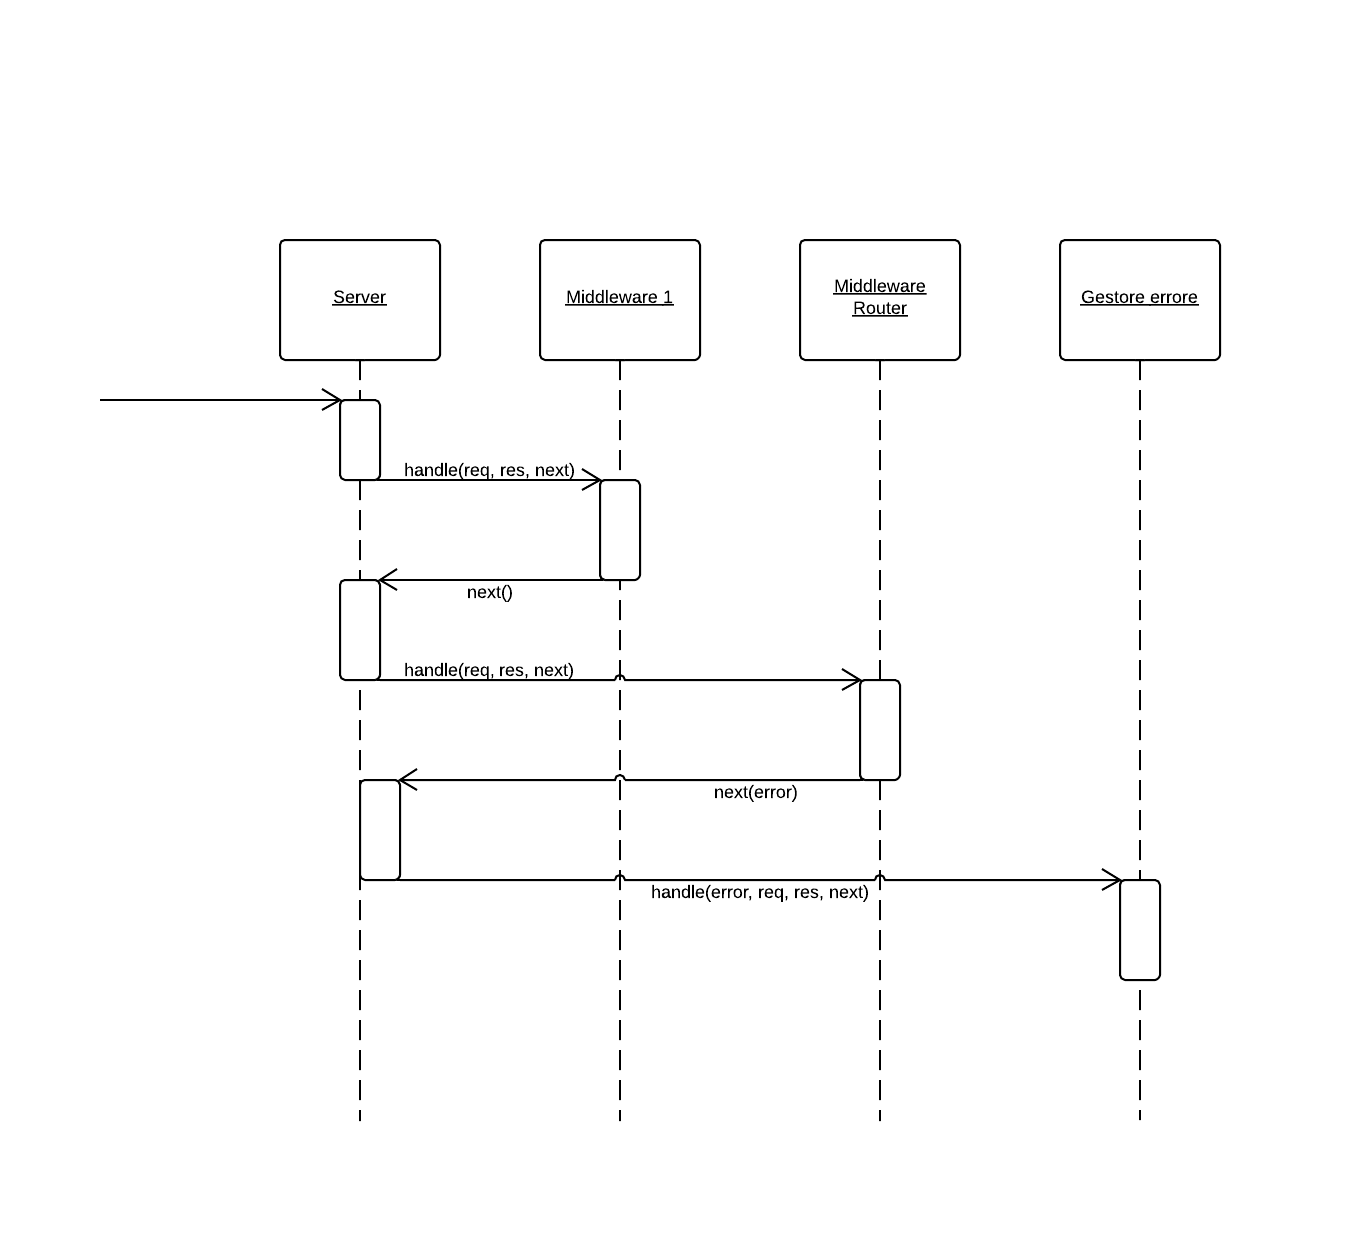
\includegraphics[scale=0.27]{scenari/Diagramma Gestione Richiesta.png}  
		\caption{Diagramma Gestione Richiesta}
	\end{center}  
\end{figure} 

Nel seguente diagramma viene mostrato il comportamento di routing, dove si intende che ogni controllore ha associato un'espressione regolare che specifica su quali richieste agisce. 
\begin{figure}[H]
	\begin{center} 
		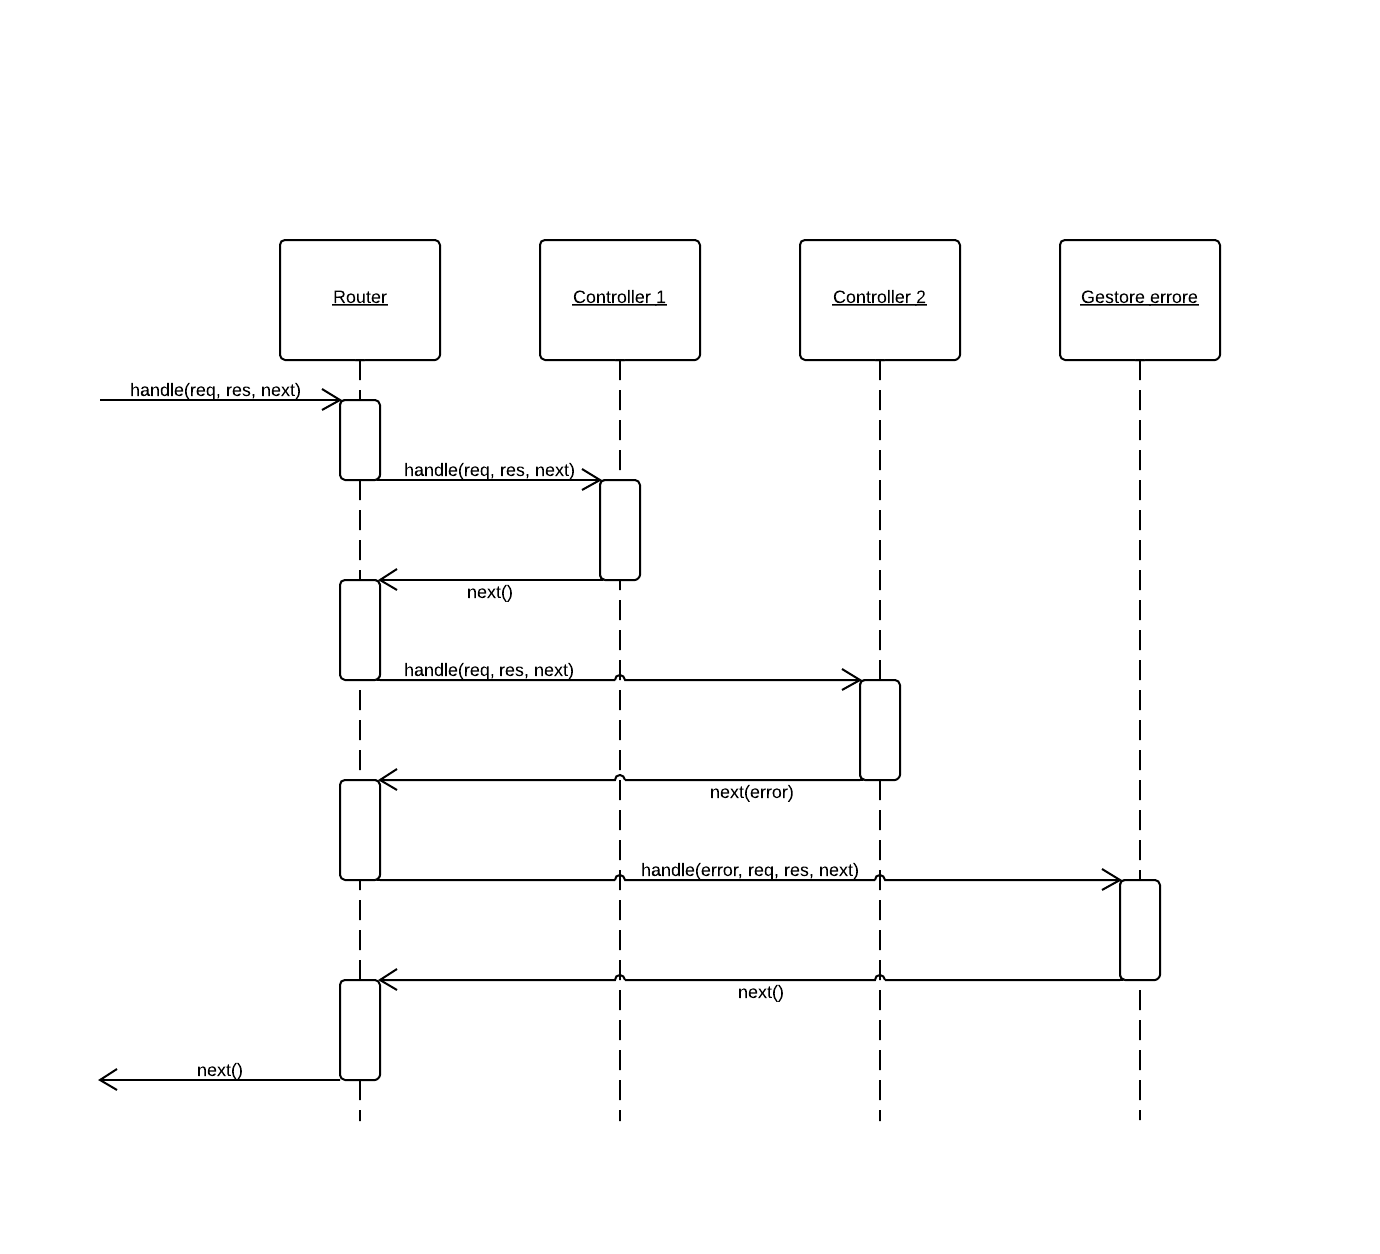
\includegraphics[scale=0.27]{scenari/Diagramma Routing Richiesta.png} 
		\caption{Diagramma Routing Richiesta}
	\end{center} 
\end{figure}

\subsection{Scenari}

\subsubsection{Fallimento vincolo ``utente autenticato''}
Per ogni richiesta bisogna verificare che il permesso dell'utente che l'ha chiesta, corrisponda al permesso che la risorsa necessita per poter essere effettuata. \\
Tale scenario rappresenta il fallimento di una richiesta richiedente come vincolo per poter essere effettuata che l'utente abbia un permesso di tipo ''utente autenticato'', dove la verifica dei permessi è gestita dal controller \emph{requireLogged} che manda un next(error) per il fallimento di tale vincolo al router il quale avrà compito di gestirlo.
\begin{figure}[H]
	\begin{center} 
		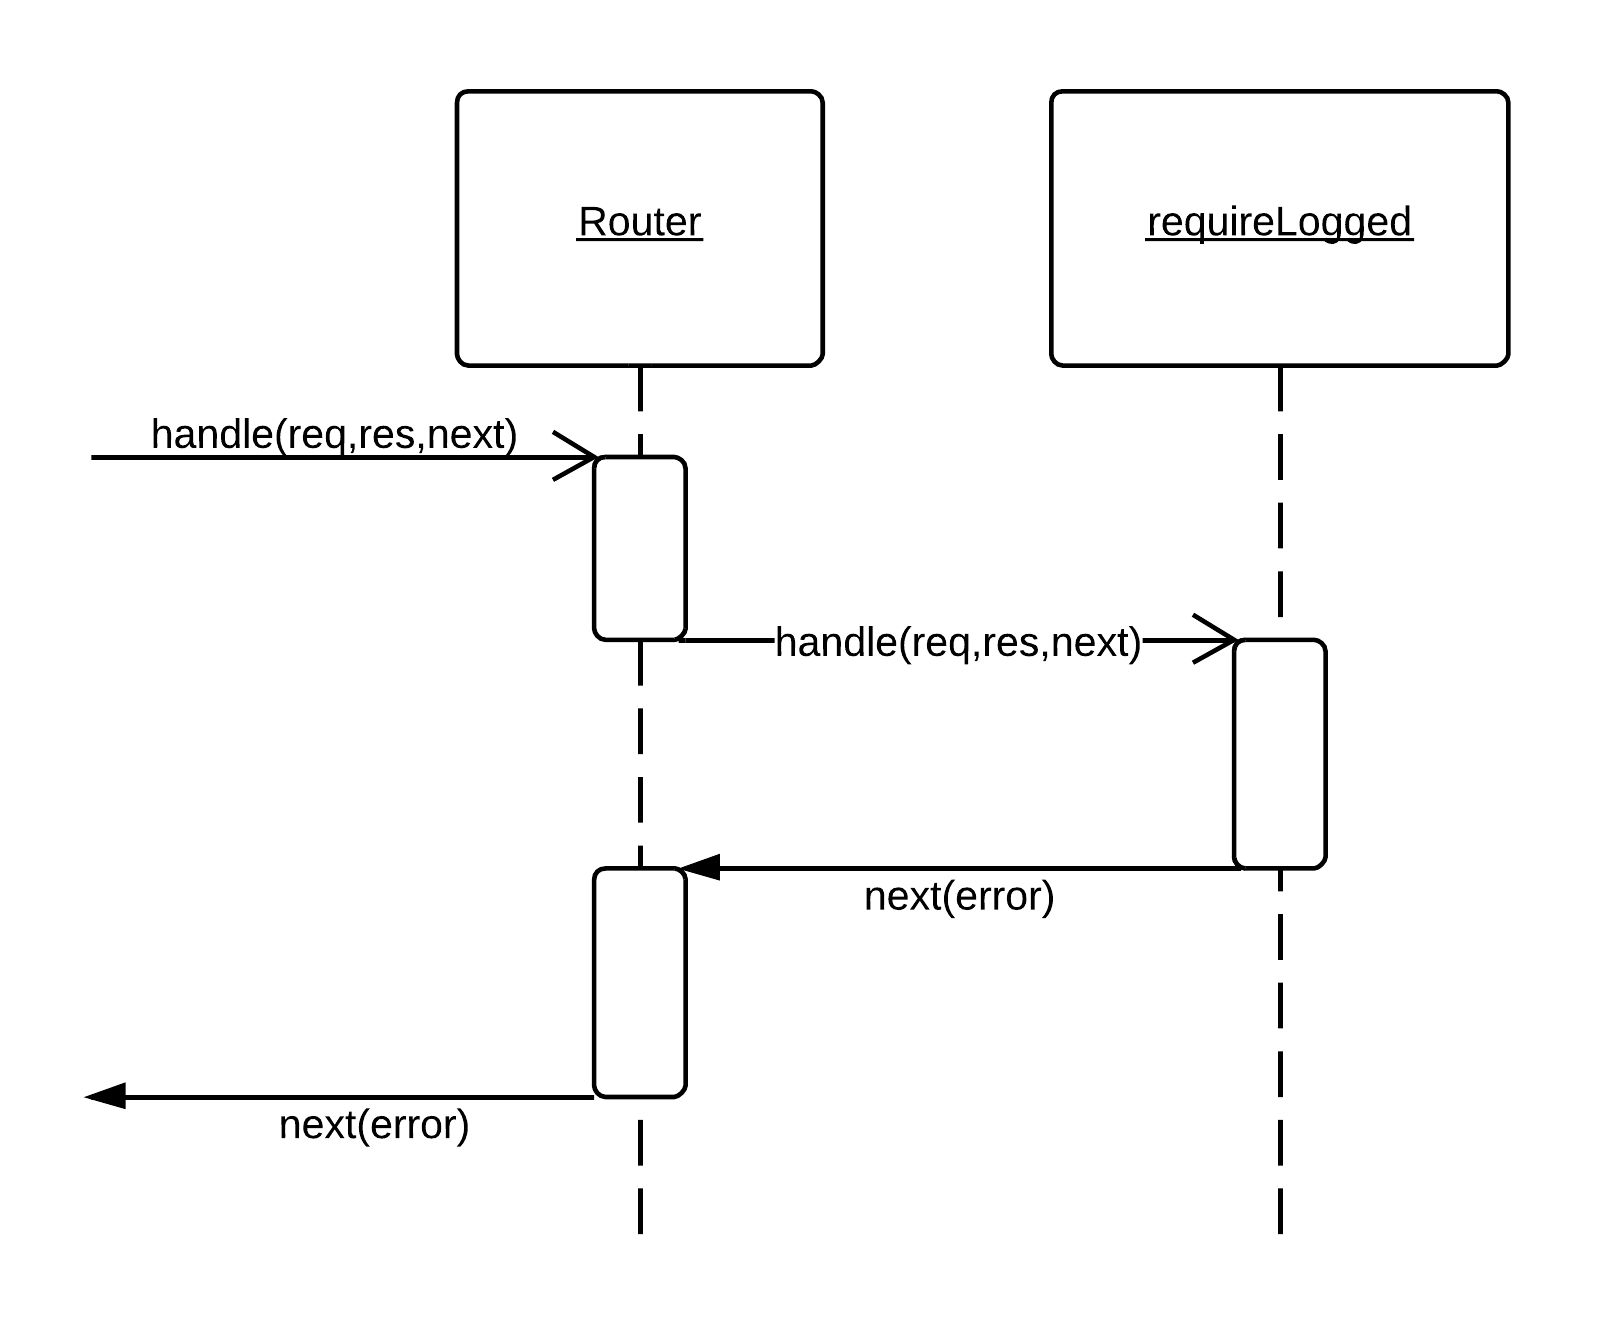
\includegraphics[scale=0.20]{scenari/requireLogged ERROR.png} 
		\caption{requireLogged ERROR}
	\end{center} 
\end{figure}

\subsubsection{Fallimento vincolo ``utente non autenticato''}
Il seguente diagramma di sequenza rappresenta lo scenario in cui fallisce la verifica del vincolo di permesso ''utente autenticato''.
La richiesta viene gestita da \emph{requireNotLogged} che verifica con esito negativo i permessi e rimanda un next(error) al router.
\begin{figure}[H]
	\begin{center} 
		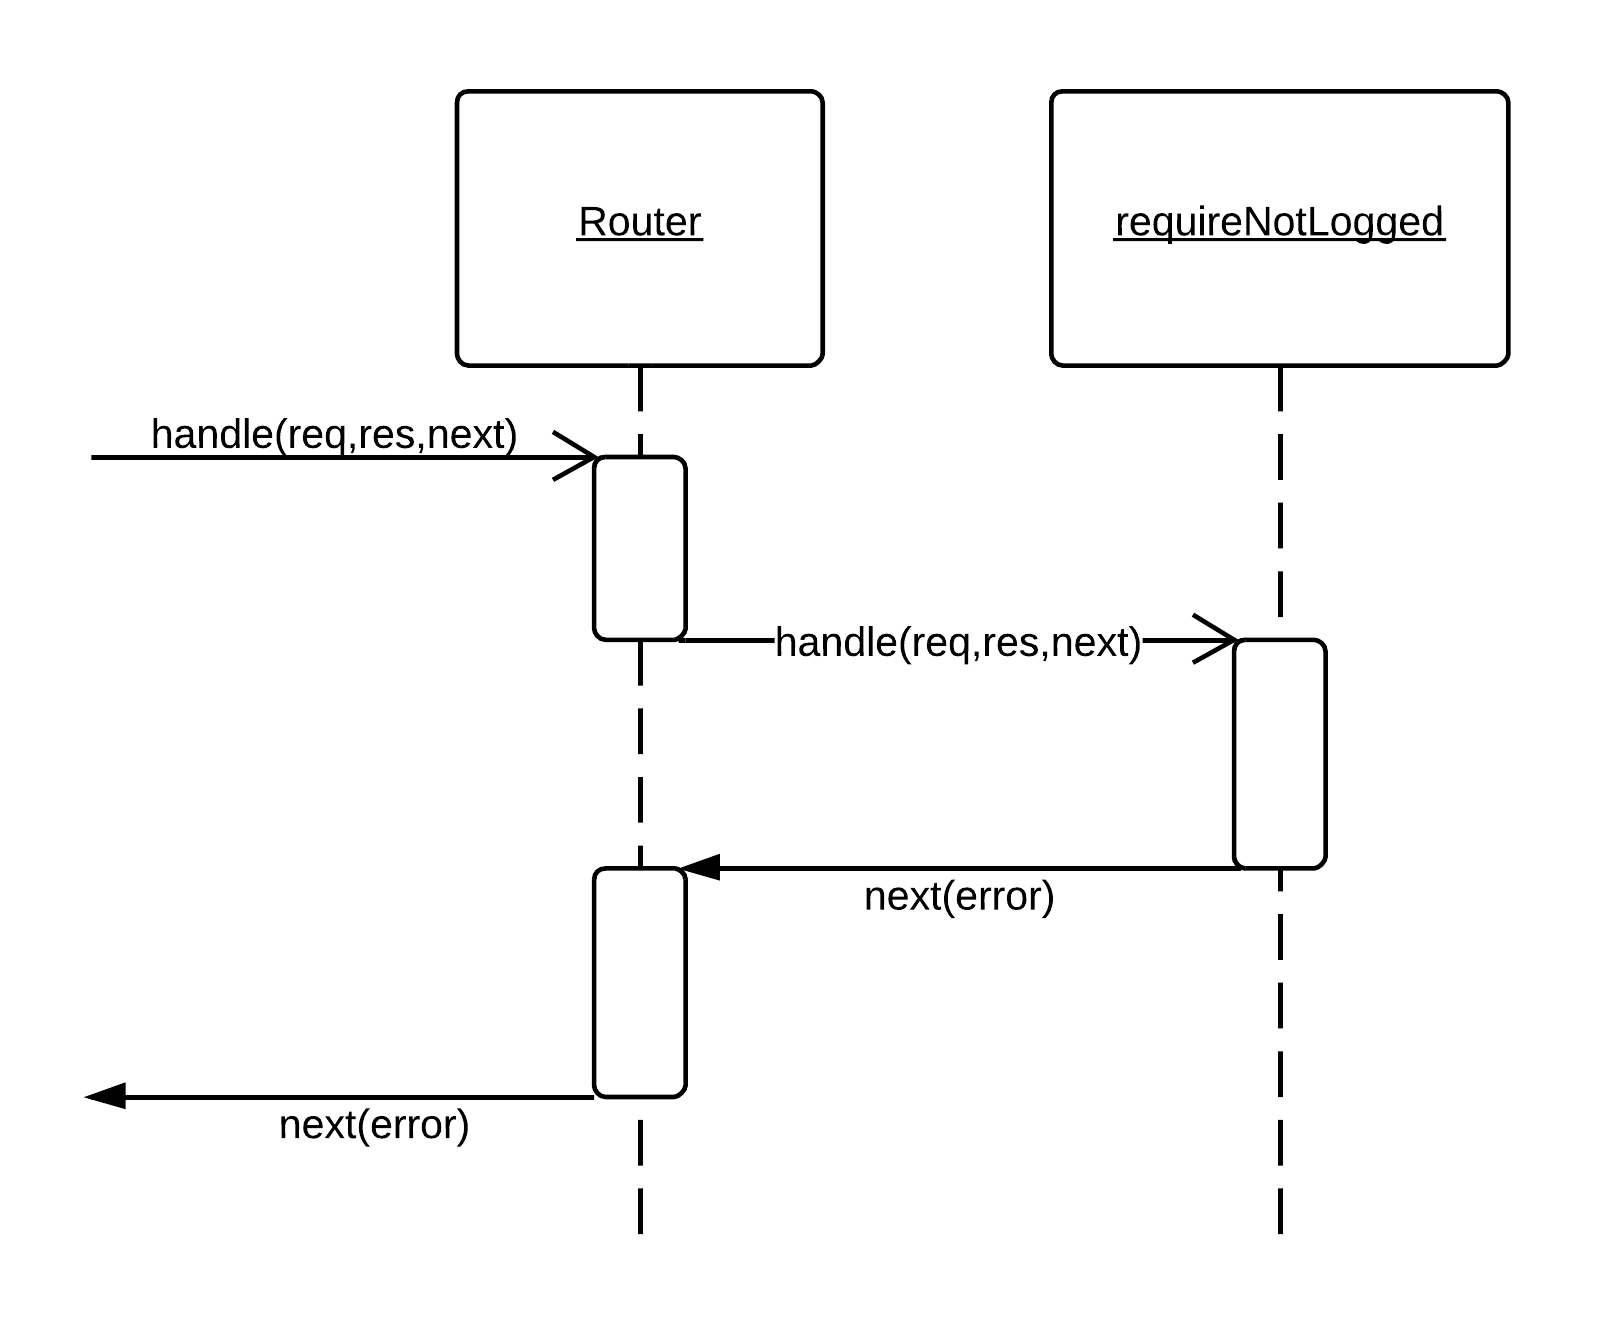
\includegraphics[scale=0.20]{scenari/requireNotLogged ERROR.png} 
		\caption{requireNotLogged ERROR}
	\end{center} 
\end{figure}

\subsubsection{Fallimento vincolo ``utente admin''}
Nel diagramma seguente viene rappresentato lo scenario in cui si richiedono permessi ''Admin'' per poter gestire la richiesta corrispondente e la verifica effettuata dal controller \emph{requireAdmin} fallisce. 
\begin{figure}[H]
	\begin{center} 
		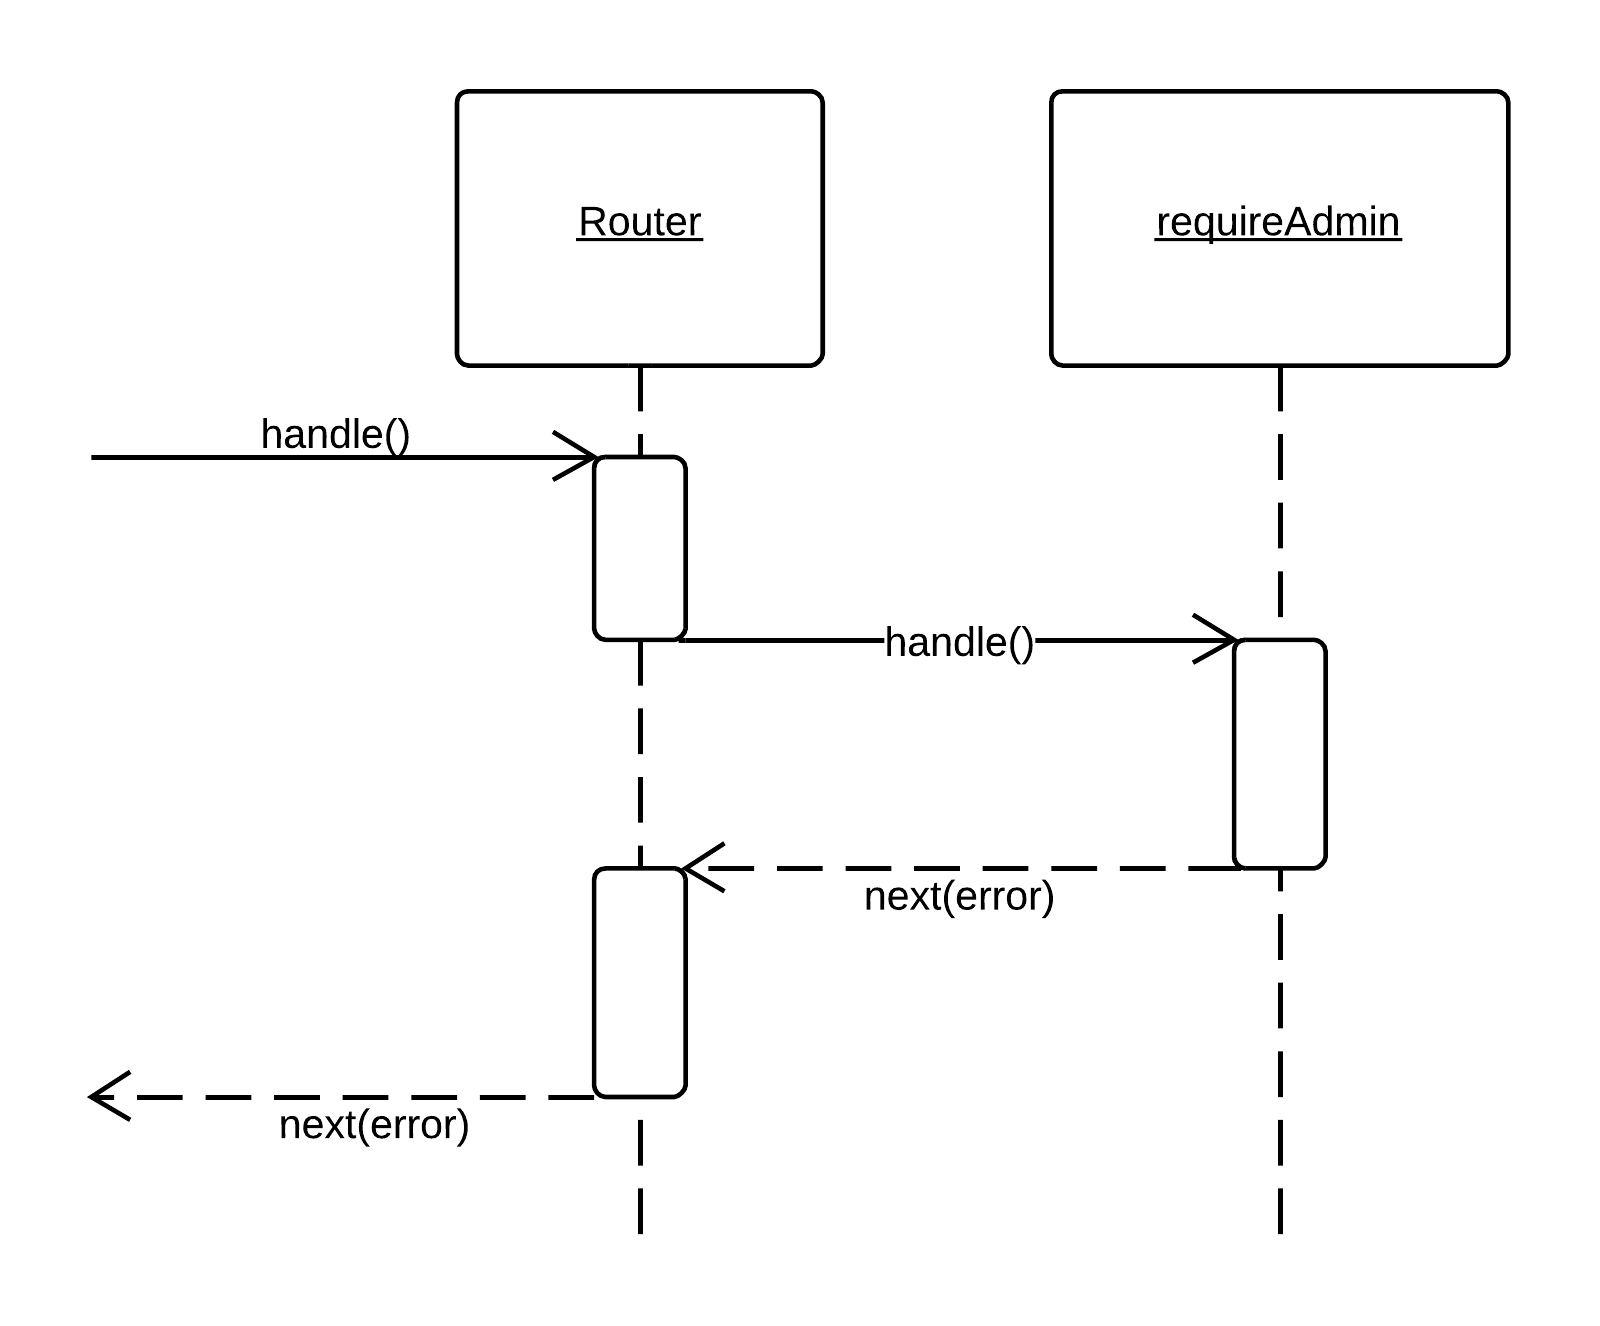
\includegraphics[scale=0.20]{scenari/requireAdmin ERROR.png} 
		\caption{requireAdmin ERROR}
	\end{center} 
\end{figure}


\subsubsection{Login POST} 
Il seguente scenario mostra la gestione di una richiesta POST per la risorsa di login, \emph{requireNotLogged} non risponde con errore, chiamando il successivo \glossario{middleware} \emph{login} che gestisce la verifica dei parametri e nell'opzione che questa fallisca, manda in risposta un next(error) che il router andrà a gestire.
\begin{figure}[H]
	\begin{center} 
		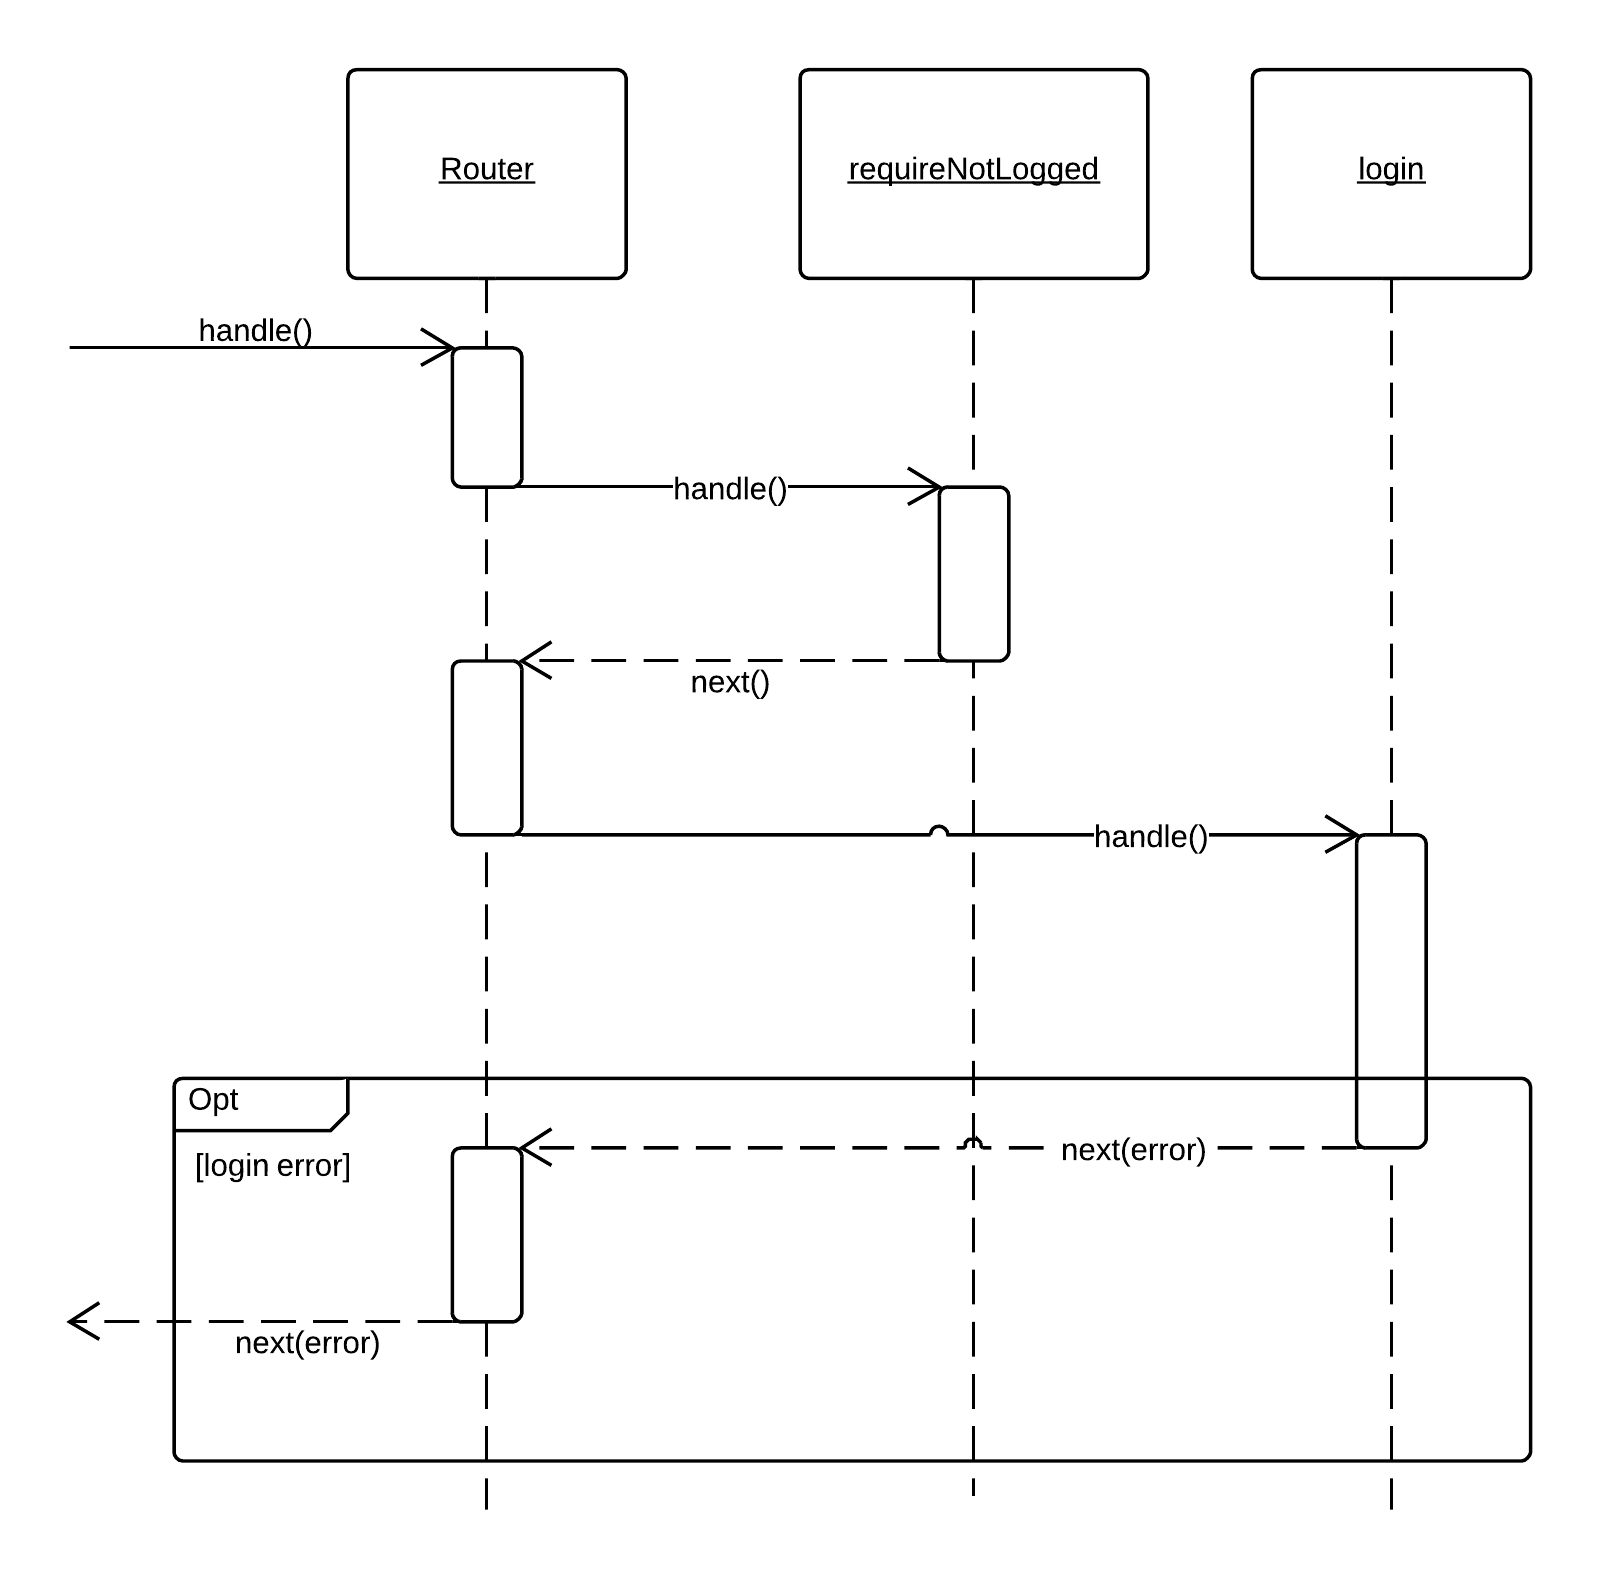
\includegraphics[scale=0.20]{scenari/login POST.png} 
		\caption{Login POST}
	\end{center} 
\end{figure} 

\subsubsection{Logout DELETE}
Il diagramma di sequenza mostra lo scenario di una richiesta DELETE per la risorsa login.
La verifica dei permessi in \emph{requireLogged} non fallisce, innescando la chiamata al successivo \glossario{middleware} \emph{logout} che gestisce l'eliminazione della risorsa.
\begin{figure}[H]
	\begin{center} 
		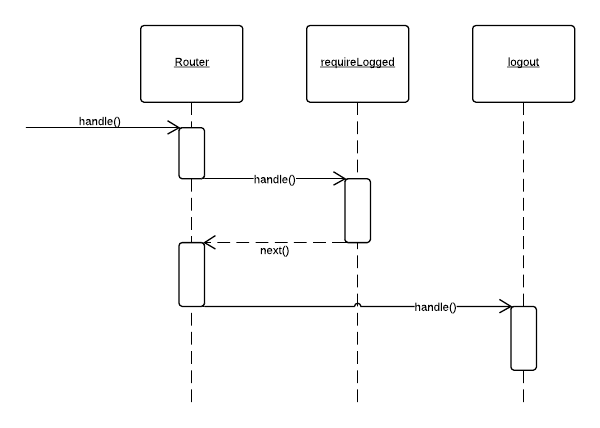
\includegraphics[scale=0.20]{scenari/logout DELETE.png} 
		\caption{Logout DELETE}
	\end{center} 
\end{figure}

\subsubsection{Profile GET} 
Il seguente diagramma rappresenta lo scenario di una richiesta GET per ottenere la risorsa Profile, la verifica dei permessi non fallisce e la richiesta viene gestita da \emph{getProfile}.
\begin{figure}[H]
	\begin{center} 
		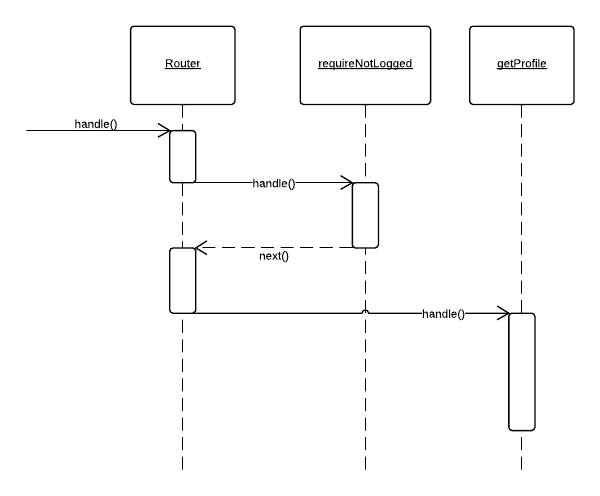
\includegraphics[scale=0.20]{scenari/Profile GET.png} 
		\caption{Profile GET}
	\end{center} 
\end{figure}

\subsubsection{Profile PUT} 
Viene rappresentato lo scenario di una richiesta PUT per la risorsa Profile, il \emph{requireLogged} non ritorna un errore, chiamando il successivo \glossario{middleware} \emph{editProfile} che gestisce la richiesta di modifica dei dati del profilo.
\begin{figure}[H]
	\begin{center} 
		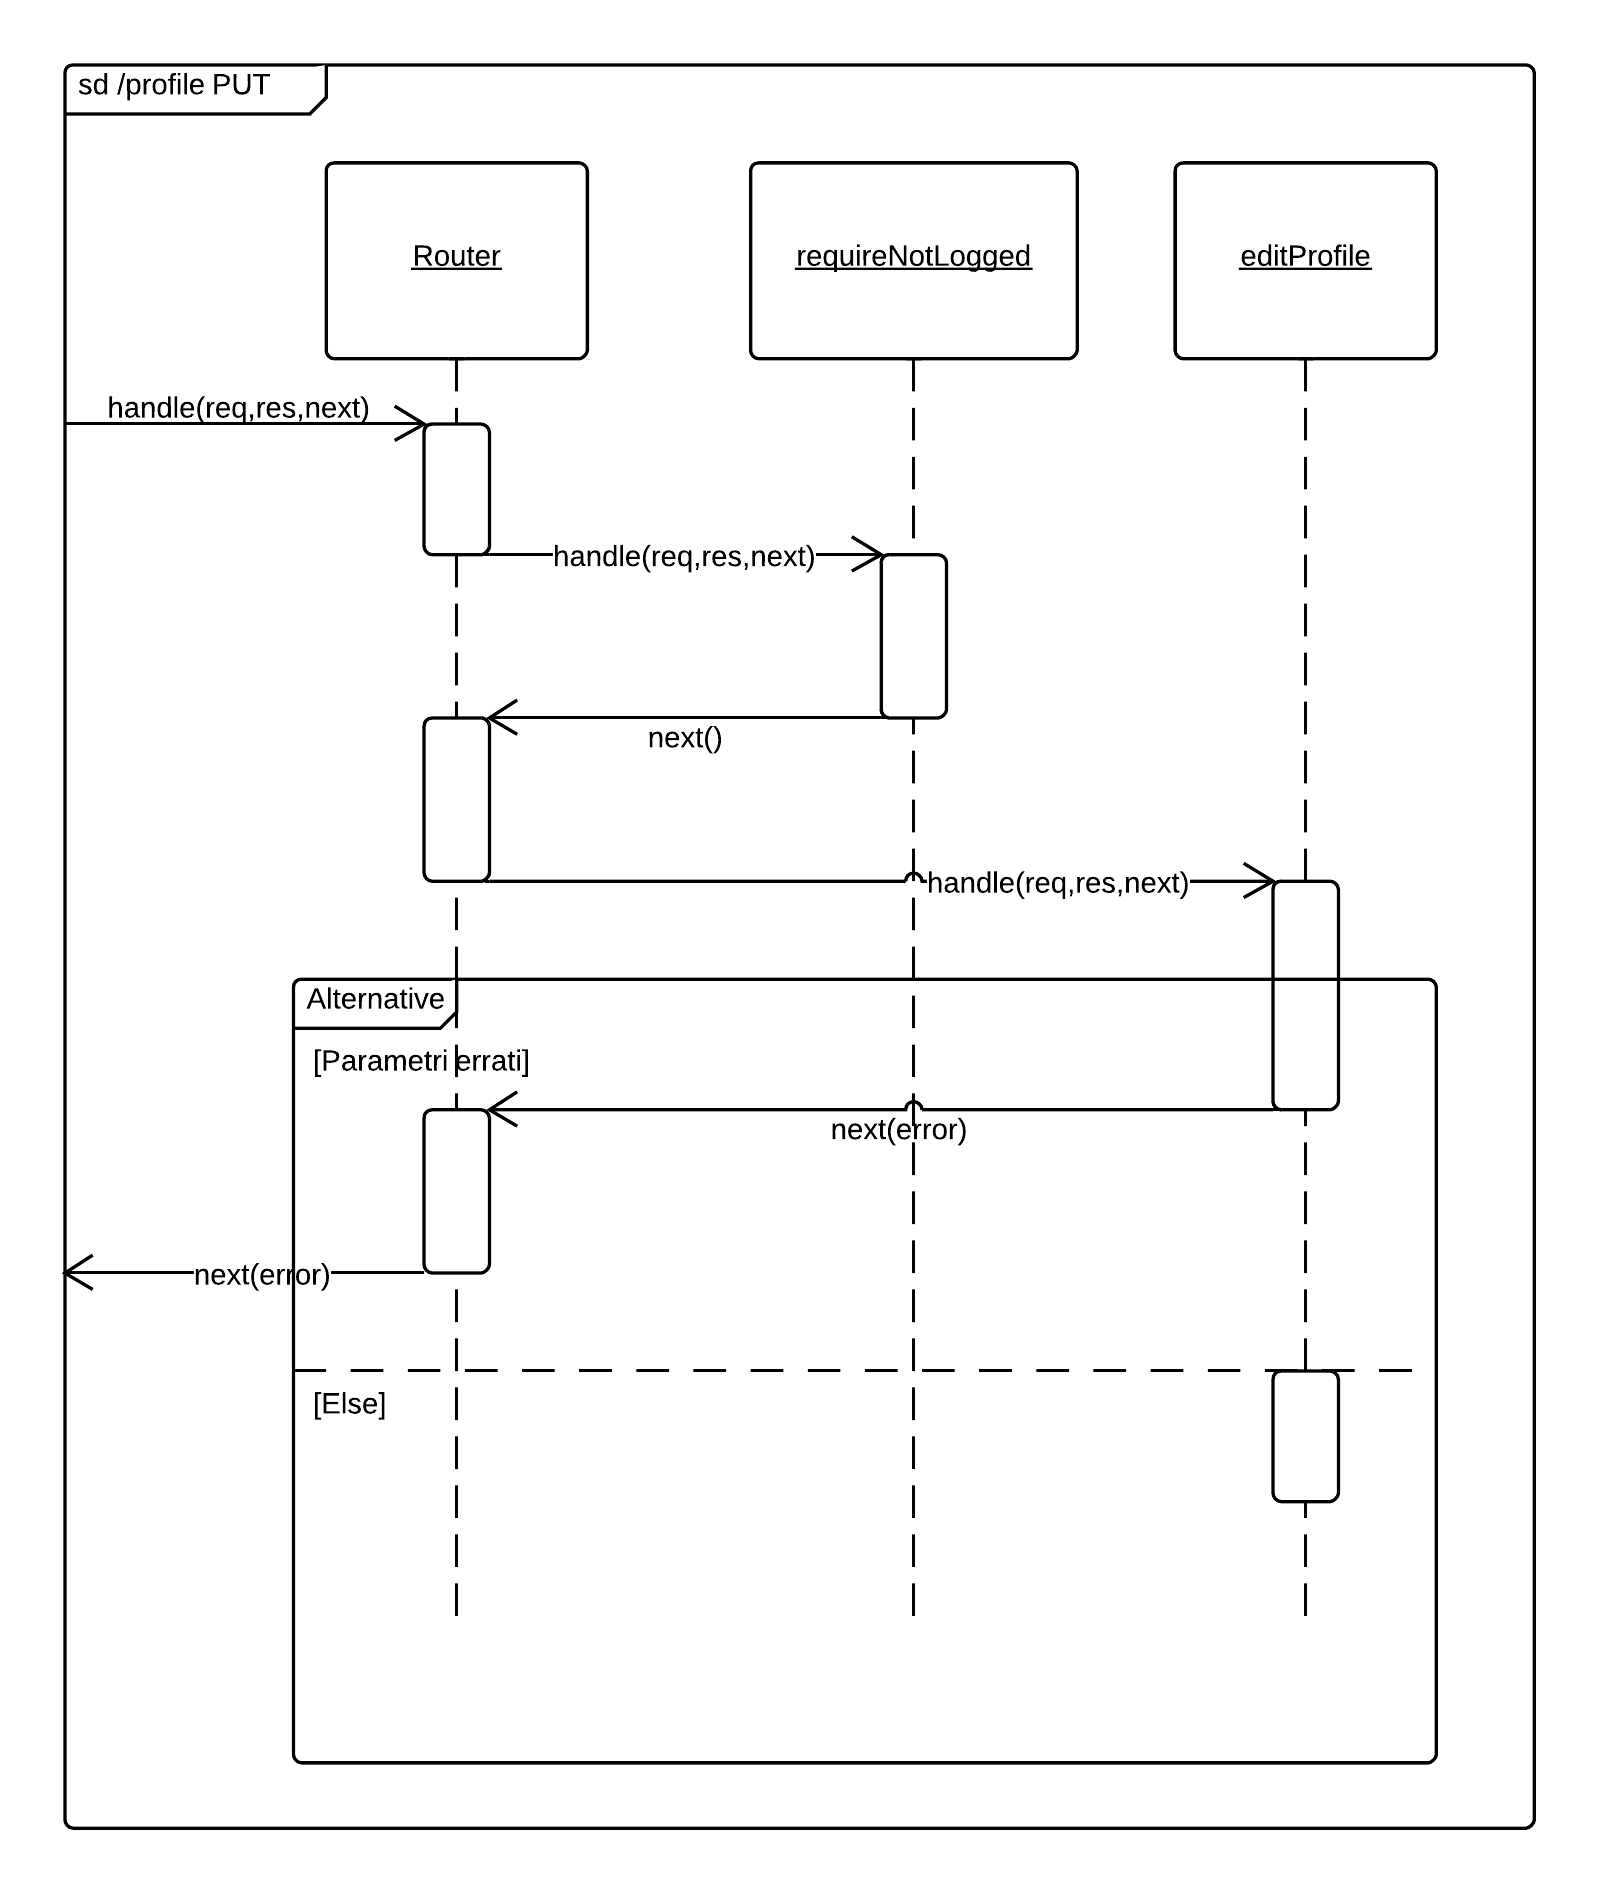
\includegraphics[scale=0.20]{scenari/Profile PUT.png} 
		\caption{Profile PUT}
	\end{center} 
\end{figure}

\subsubsection{Password Forgot POST} 
Viene rappresentato lo scenario di una richiesta POST per la risorsa password forgot, il \emph{requireNotLogged} non risponde errore e il controllo passa a \emph{requirePasswordReset} che gestisce la richiesta.
\begin{figure}[H]
	\begin{center} 
		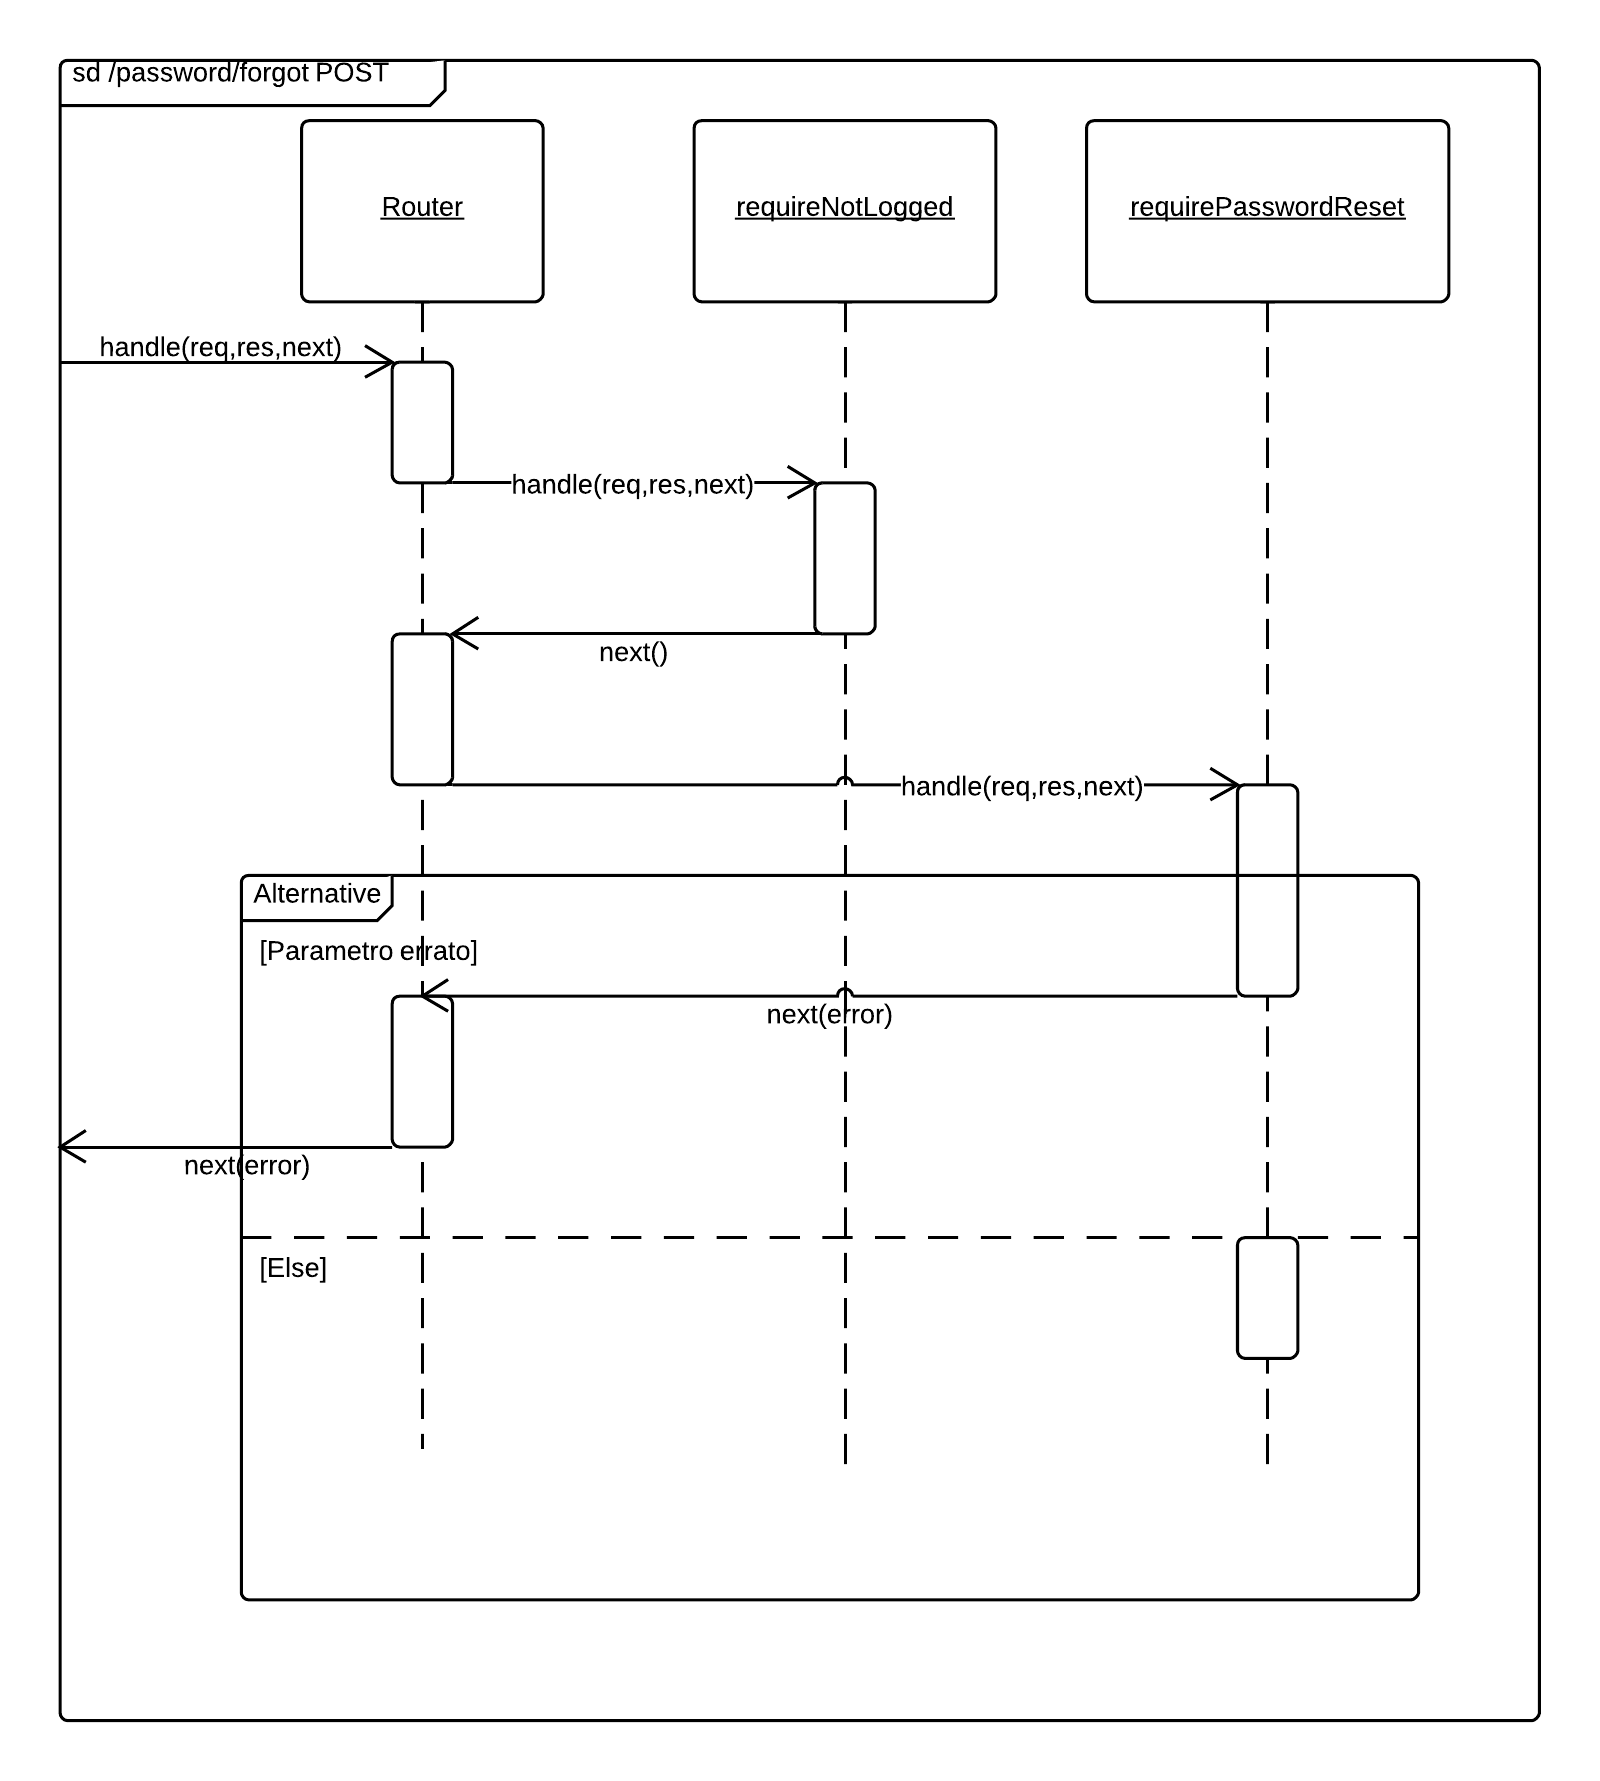
\includegraphics[scale=0.20]{scenari/Password Forgot POST.png} 
		\caption{Password Forgot POST}
	\end{center} 
\end{figure}

\subsubsection{Users GET}
Viene rappresentato nel seguente diagramma di sequenza lo scenario di una richiesta GET per la risorsa user, \emph{requireAdmin} non fallisce ed il controllo viene passato a \emph{getUsers} che gestisce la richiesta.
\begin{figure}[H]
	\begin{center} 
		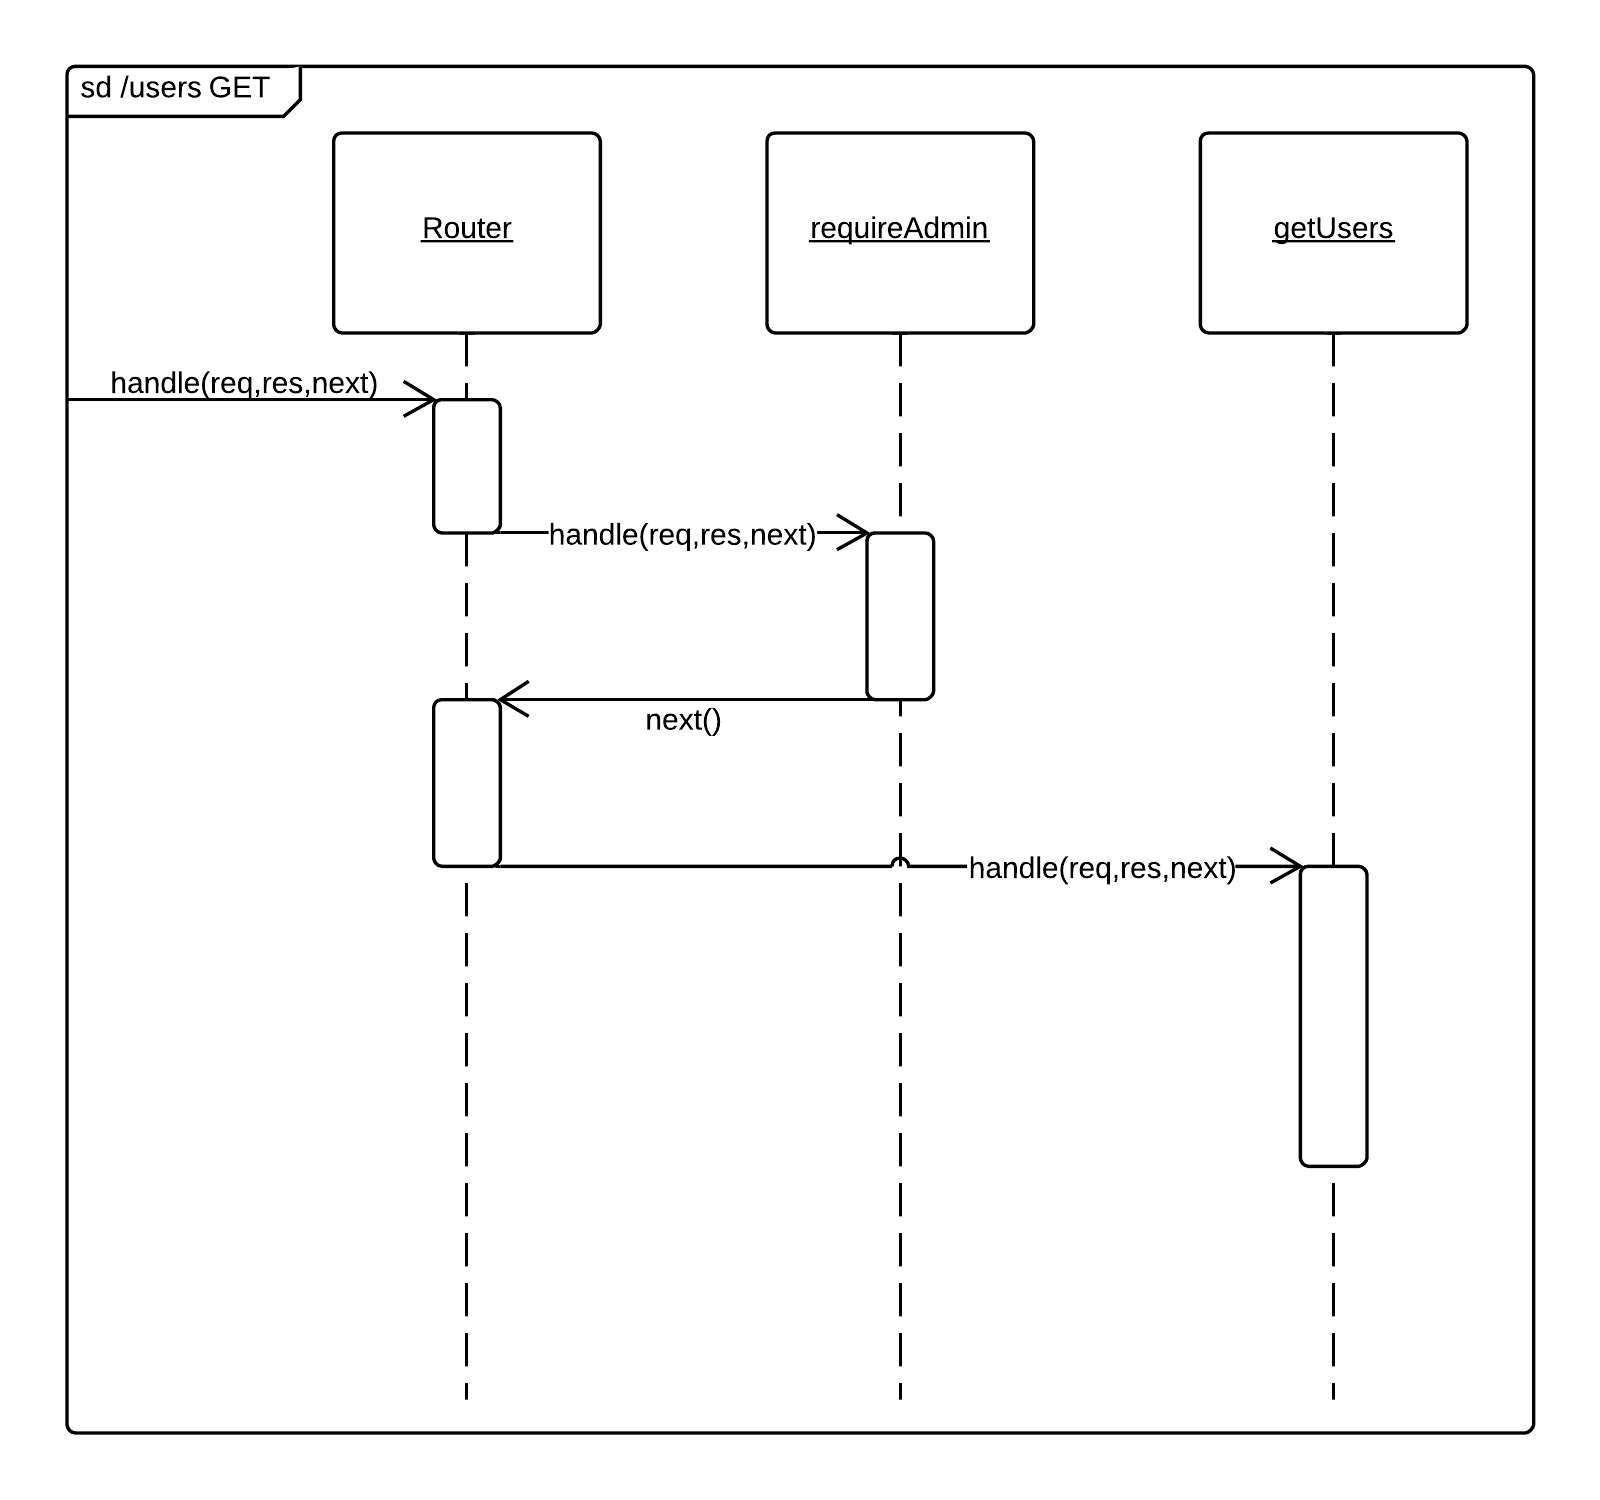
\includegraphics[scale=0.20]{scenari/Users GET.png} 
		\caption{Users GET}
	\end{center} 
\end{figure}

\subsubsection{Users POST} 
Il seguente diagramma di sequenza rappresenta lo scenario di una richiesta POST per la risorsa user, la verifica di \emph{requireLogged} dei permessi utente non fallisce e viene passato il controllo a \emph{createUser} che gestisce la richiesta di creazione di un nuovo user.
\begin{figure}[H]
	\begin{center} 
		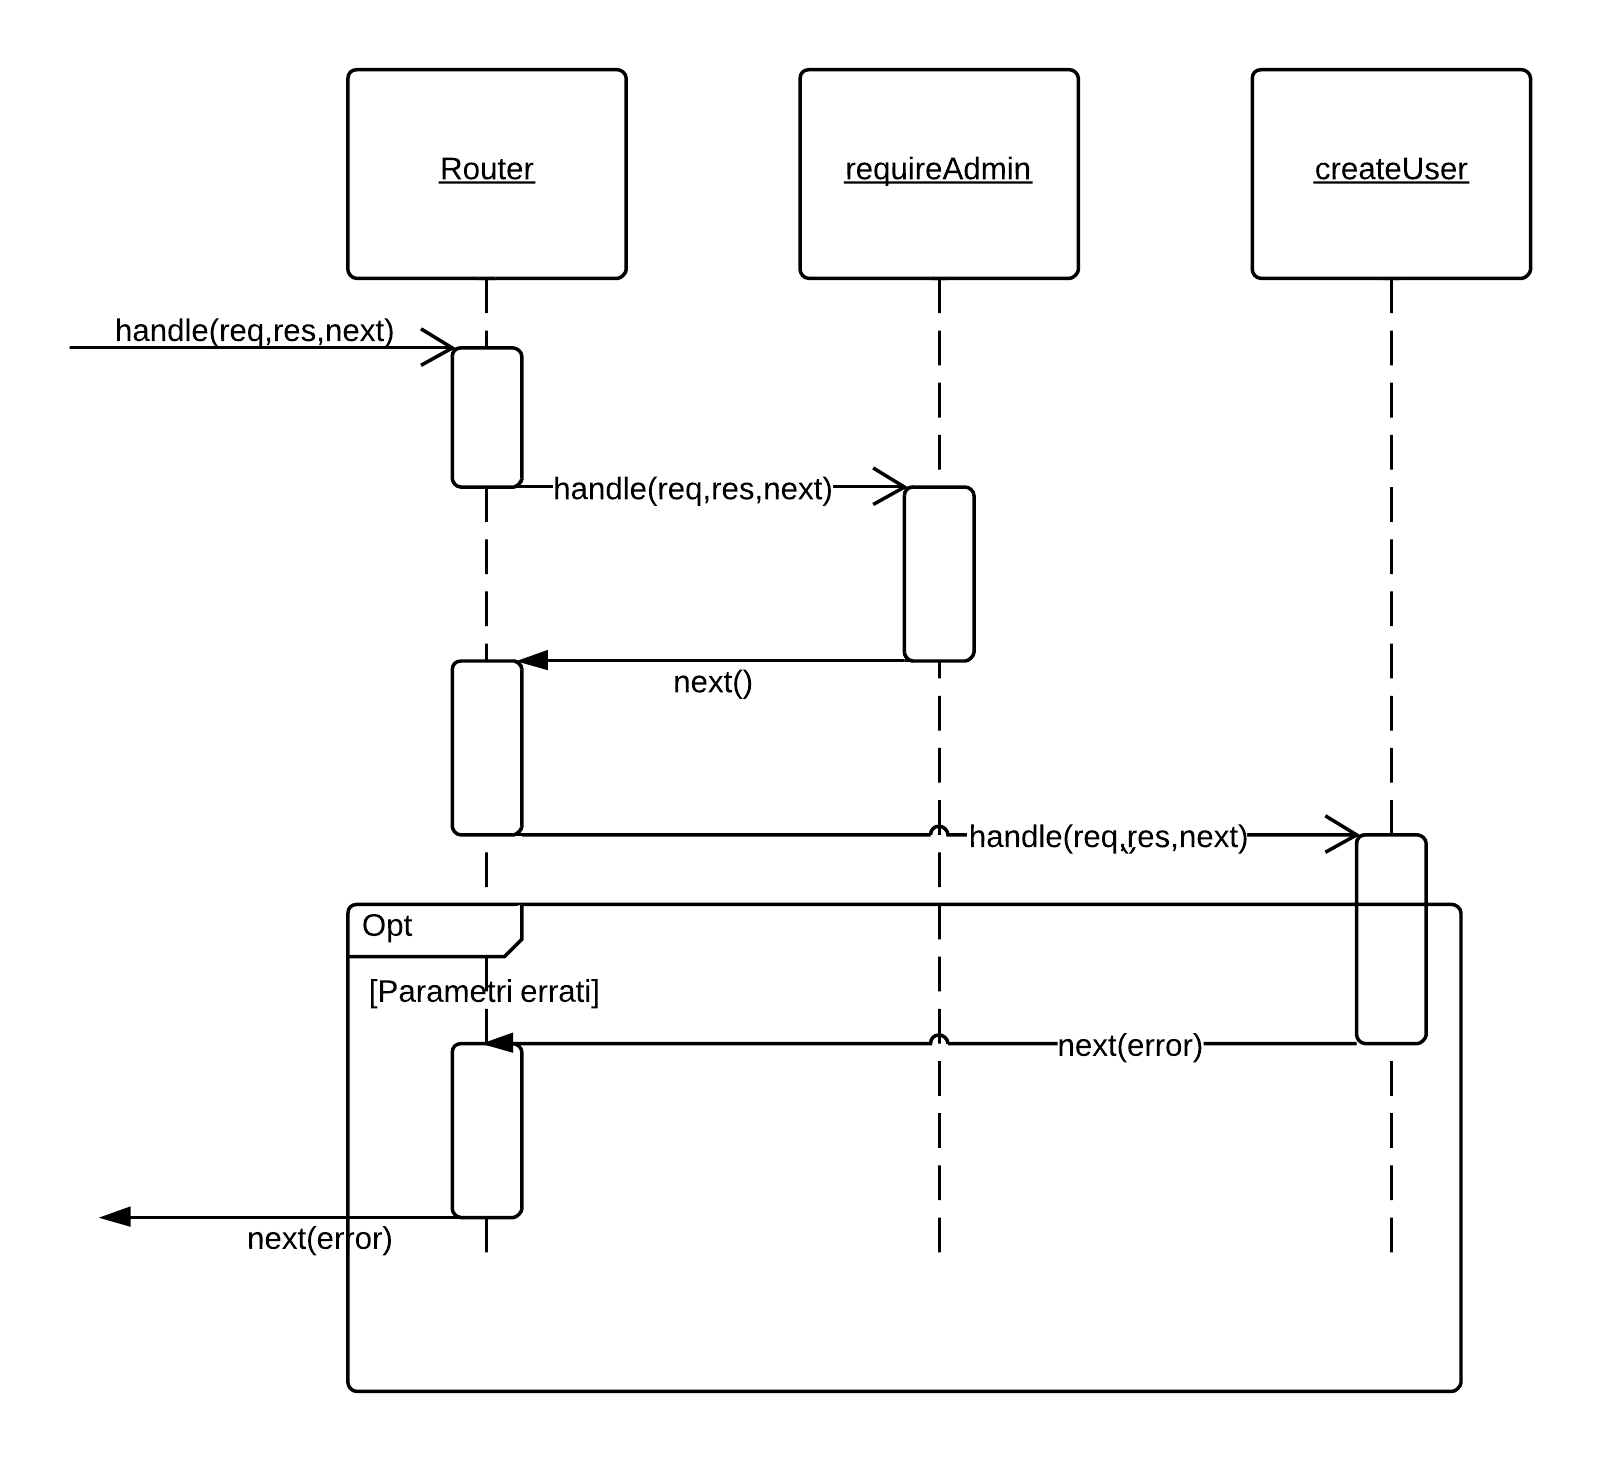
\includegraphics[scale=0.20]{scenari/Users POST.png} 
		\caption{Users POST}
	\end{center} 
\end{figure}

\subsubsection{Users Id GET} 
Lo scenario rappresenta una richiesta GET di una risorsa User id, vengono verificati i permessi attraverso \emph{requireAdmin} che passa il controllo a \emph{getUser} dandogli come attributo l'id dell'user da restituire.
\begin{figure}[H]
	\begin{center} 
		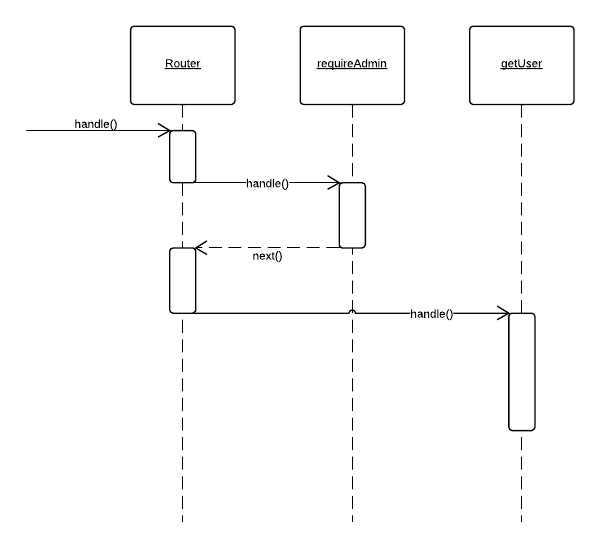
\includegraphics[scale=0.20]{scenari/Users Id GET.png} 
		\caption{Users Id GET}
	\end{center} 
\end{figure}

\subsubsection{Users Id PUT} 
Nel seguente diagramma di sequenza viene rappresentato lo scenario di una richiesta PUT per la risorsa User id nel quale \emph{requireAdmin} non restituisce un errore e passa il controllo a \emph{editUser} che gestisce la richiesta di modifica dati dell'user corrispondente all'userId che gli è stato passato come attributo.
\emph{EditUser} verifica inoltre che l'userId passatogli come attributo non corrisponda all'id dello stesso user che ha effettuato la richiesta o corrisponda ad un id di un superAdmin, altrimenti risponderà con un errore.
\begin{figure}[H]
	\begin{center} 
		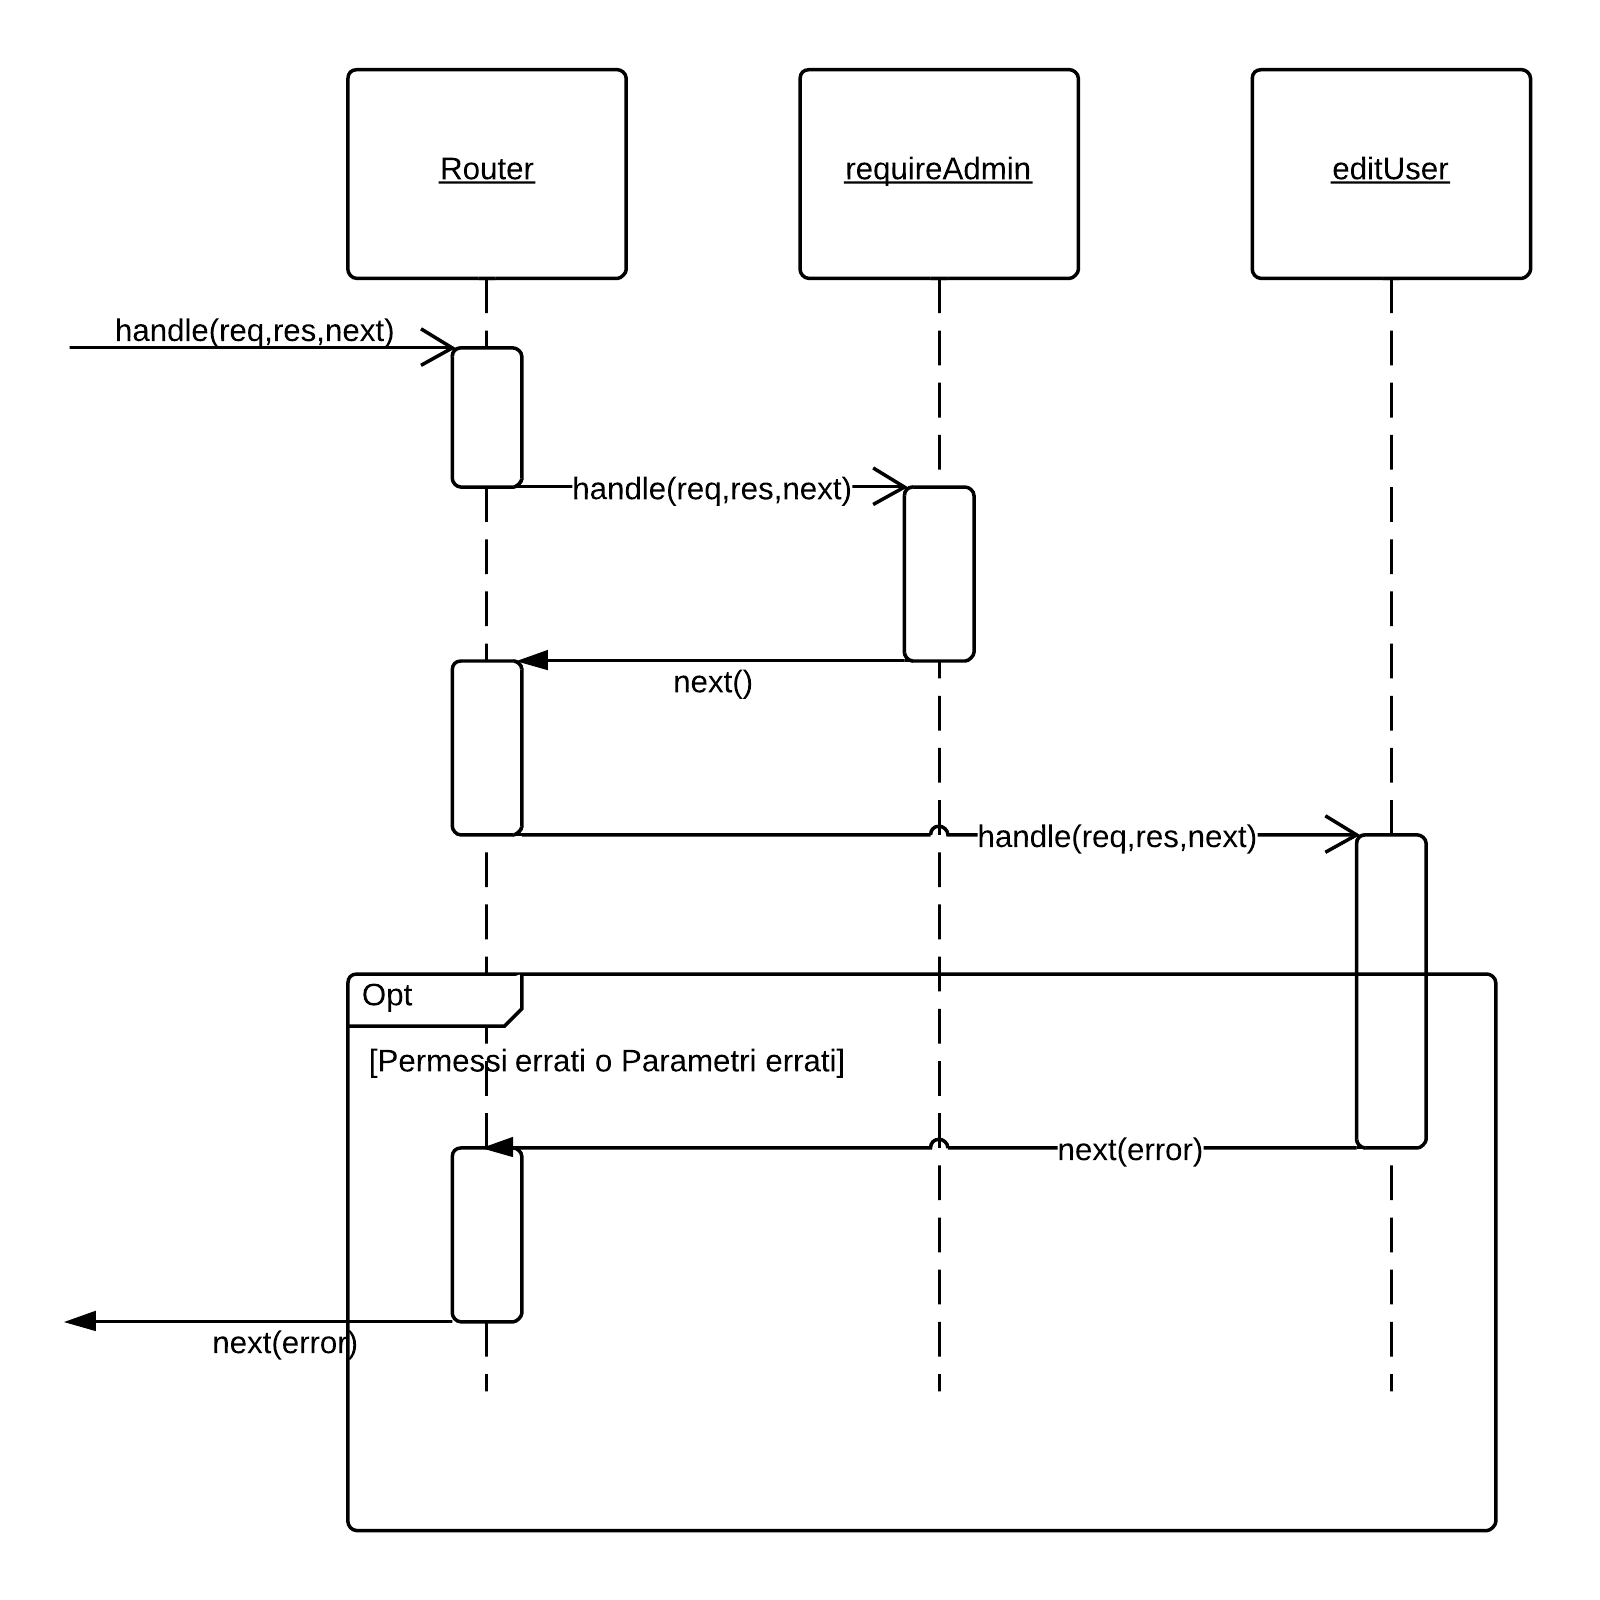
\includegraphics[scale=0.20]{scenari/Users Id PUT.png} 
		\caption{Users Id POST}
	\end{center} 
\end{figure}

\subsubsection{Users Id DELETE} 
Il diagramma di sequenza rappresenta lo scenario di una richiesta DELETE per la risorsa user id, \emph{requireAdmin} non restituisce un errore e la richiesta viene gestita da \emph{deleteUser} per procede con l'eliminazione dell'user cui id gli è stato passato come attributo.
Nell'opzione che l'id passatogli corrisponda all'id dell'utente che ha effettuato la richiesta o ad un id di un superAdmin, \emph{deleteUser} restituisce un next(error).
\begin{figure}[H]
	\begin{center} 
		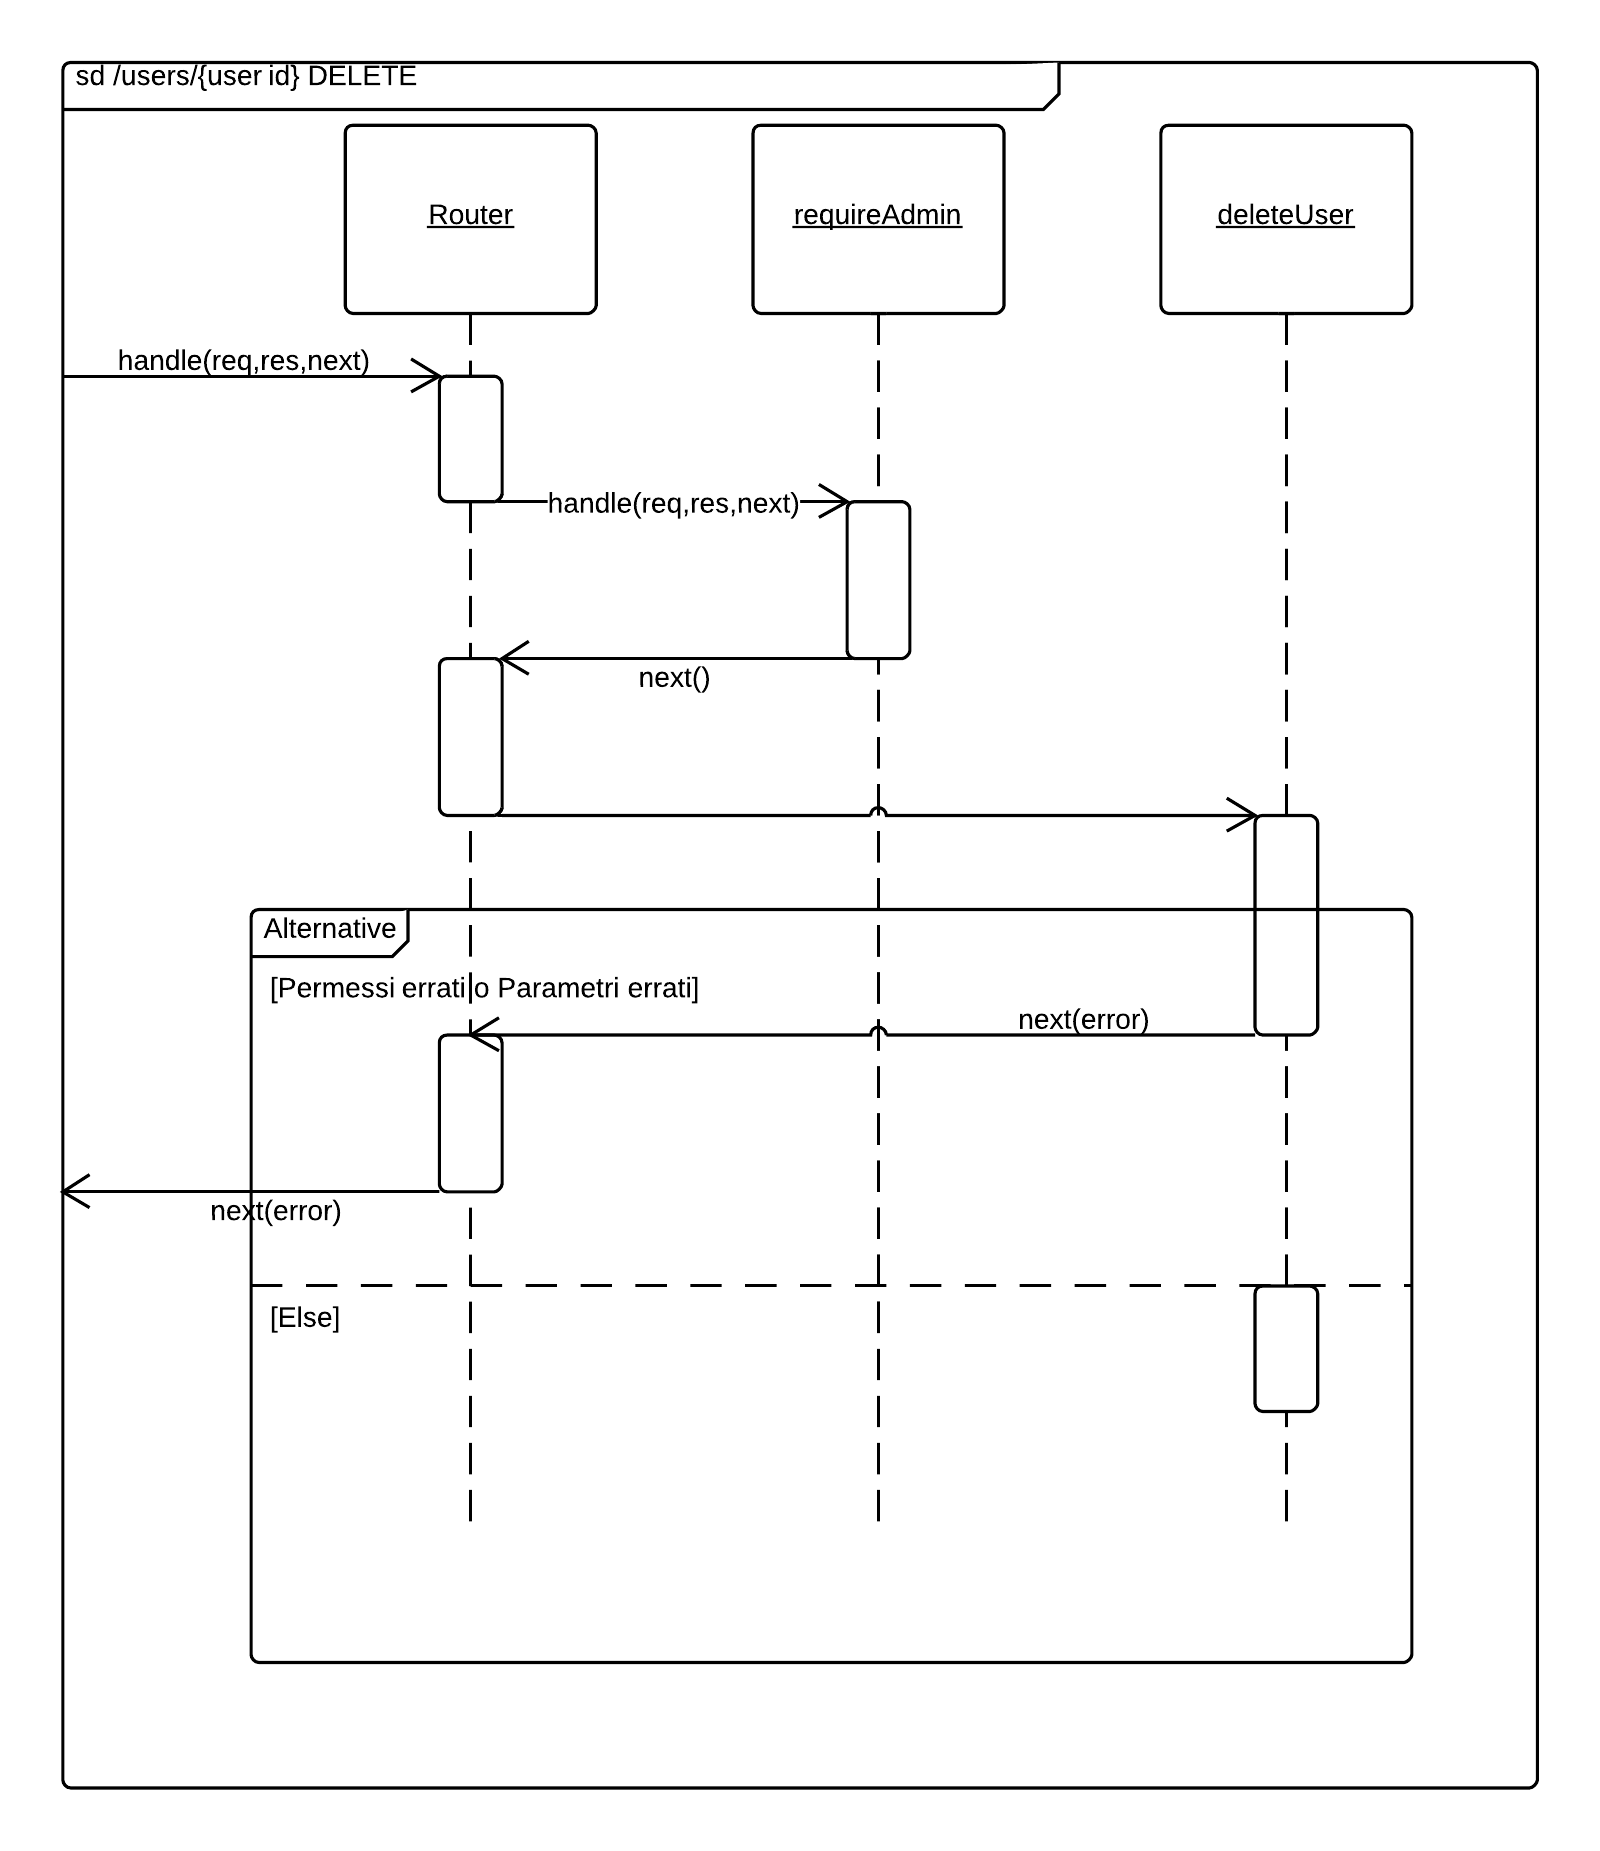
\includegraphics[scale=0.20]{scenari/Users Id DELETE.png} 
		\caption{Users Id DELETE}
	\end{center} 
\end{figure}

\subsubsection{Collection GET} 
Il diagramma seguente rappresenta lo scenario di una richiesta GET per la risorsa collection, il controller \emph{requireLogged} innescherà la chiamata del successivo controller \emph{listCollection} che gestirà la richiesta di restituzione della lista di \glossario{Collection}.
\begin{figure}[H]
	\begin{center} 
		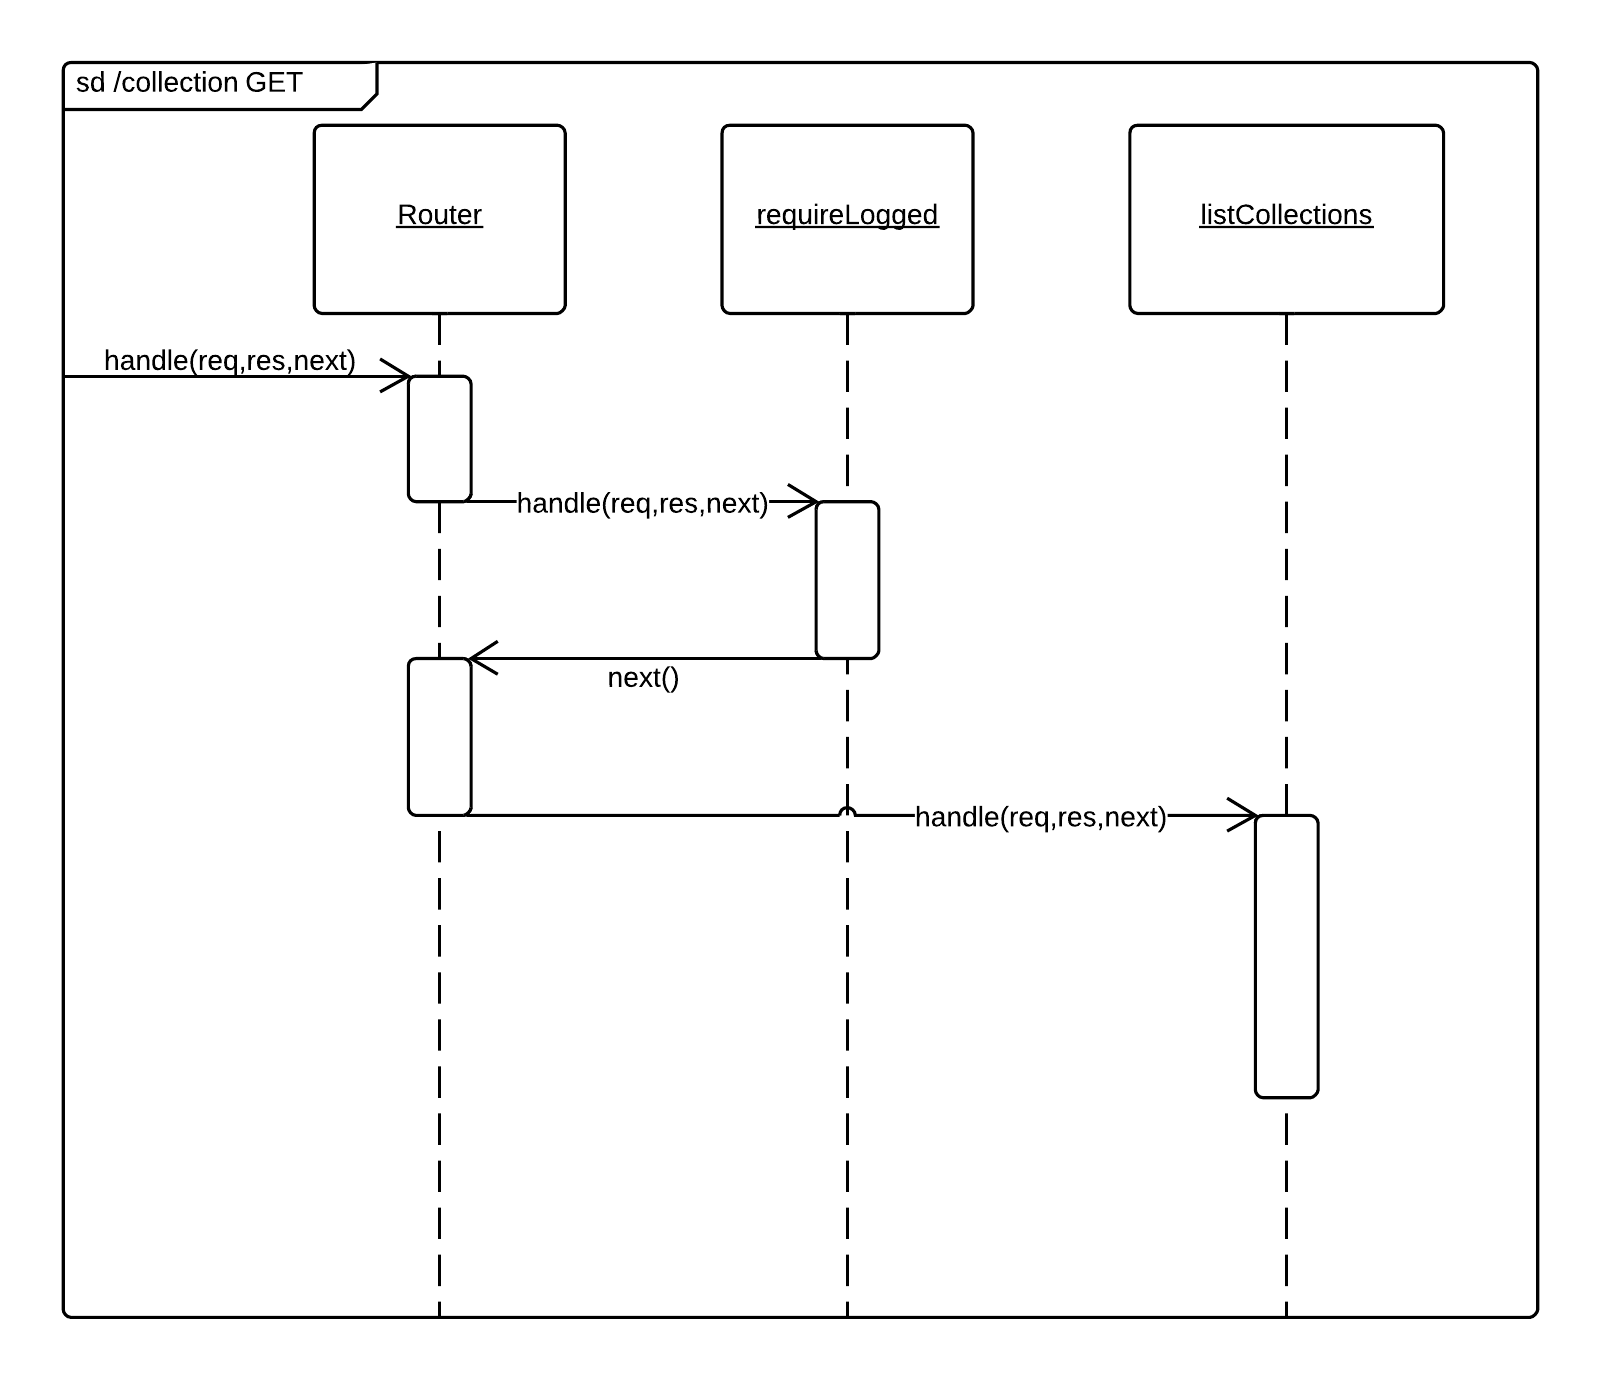
\includegraphics[scale=0.20]{scenari/Collection GET.png} 
		\caption{Collection GET}
	\end{center} 
\end{figure}

\subsubsection{Collection Name GET} 
Il diagramma seguente rappresenta lo scenario di una richiesta GET per la risorsa collection Name, il controller \emph{requireLogged} innescherà la chiamata del successivo controller \emph{indexPage} al quale verrà passato come parametro l'id della \glossario{Collection} per la restituzione dell'index page corrispondente.
\begin{figure}[H]
	\begin{center} 
		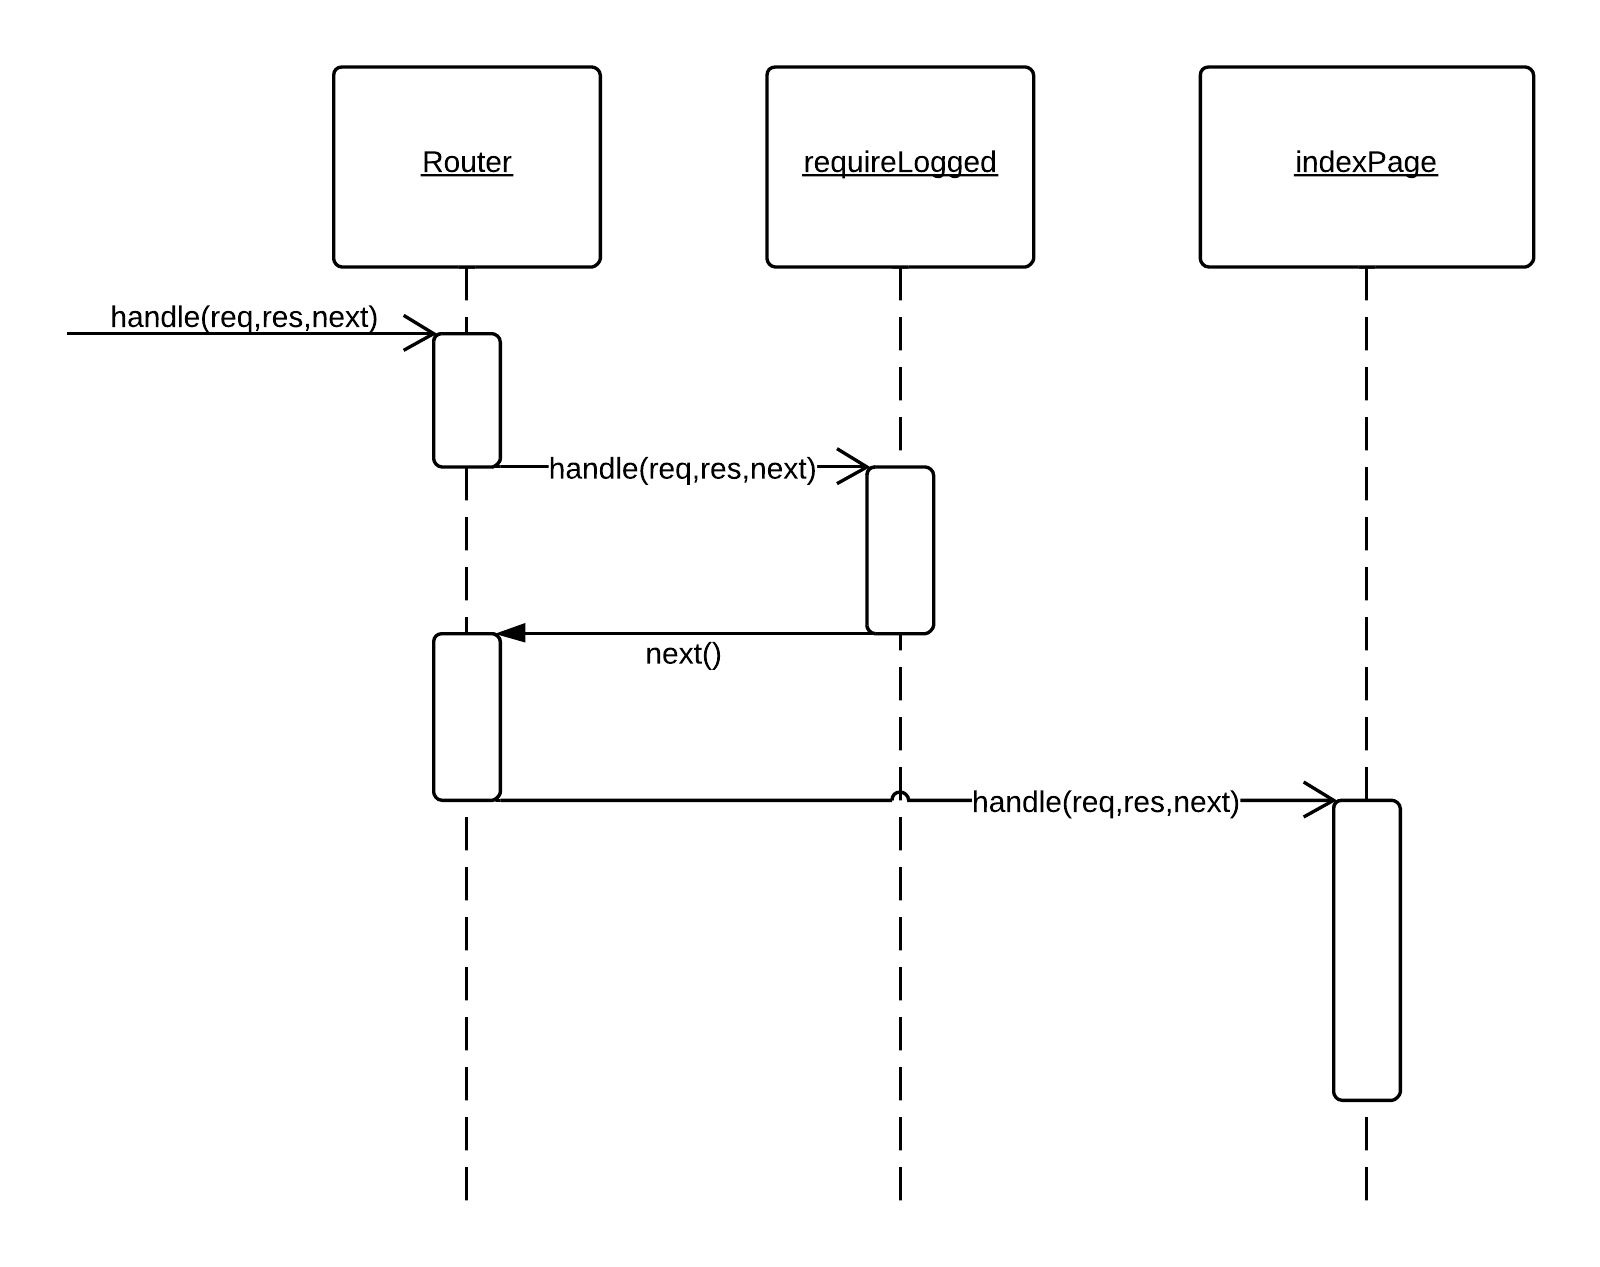
\includegraphics[scale=0.20]{scenari/Collection Name GET.png} 
		\caption{Collection Name GET}
	\end{center} 
\end{figure}

\subsubsection{Collection Name Document GET} 
Il diagramma di sequenza rappresenta lo scenario di una richiesta GET per la risorsa collection name document, nel quale al controller \emph{showpage} viene passato l'id del document di cui mostrare la show page.
\begin{figure}[H]
	\begin{center} 
		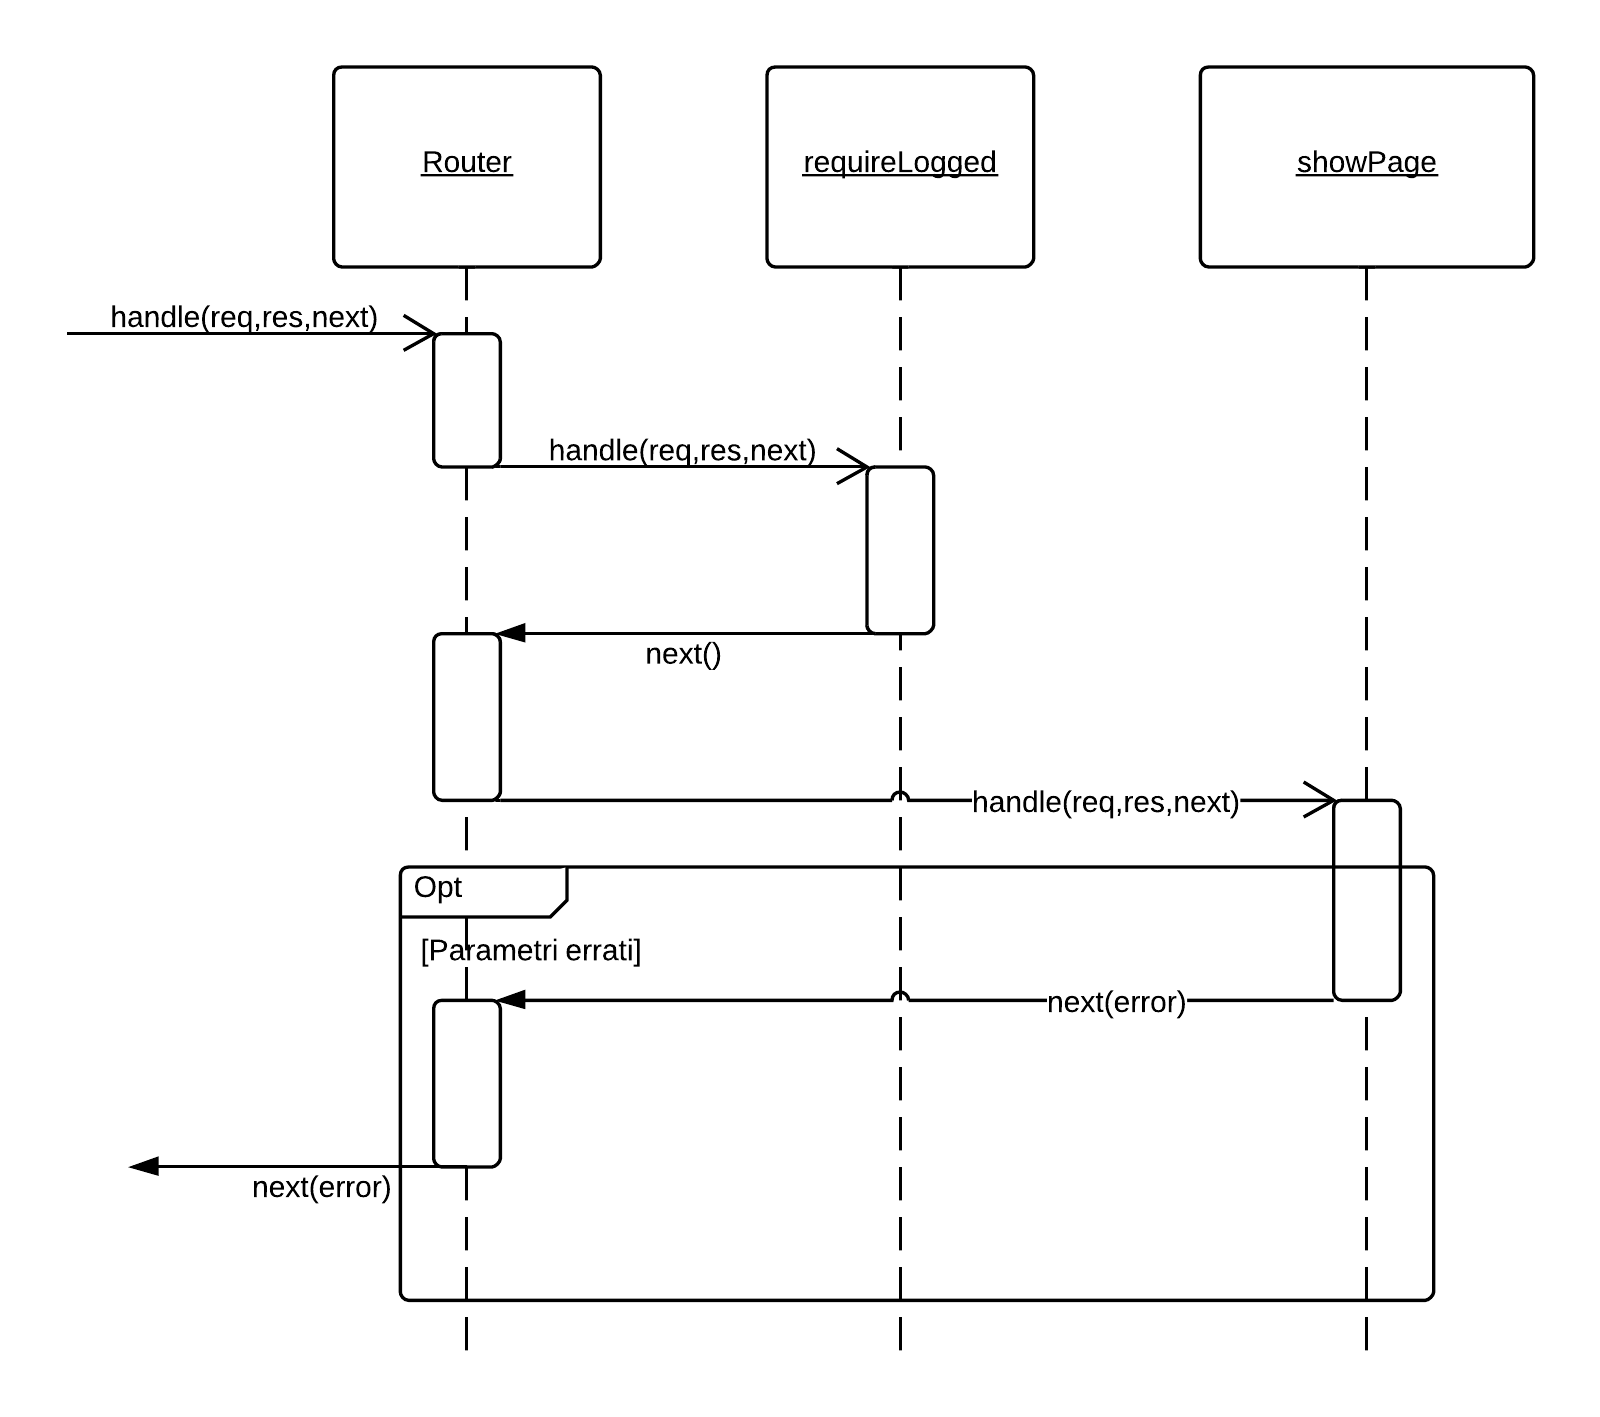
\includegraphics[scale=0.20]{scenari/Collection Name Document GET.png} 
		\caption{Collection Name Document GET}
	\end{center} 
\end{figure}

\subsubsection{Collection Name Document PUT}
Il seguente diagramma rappresenta lo scenario di una richiesta POST su una risorsa collection name document, il controller \emph{requireAdmin} non risponde con errore e viene passato il controllo a \emph{editDocument} che gestirà la richiesta.
\begin{figure}[H]
	\begin{center} 
		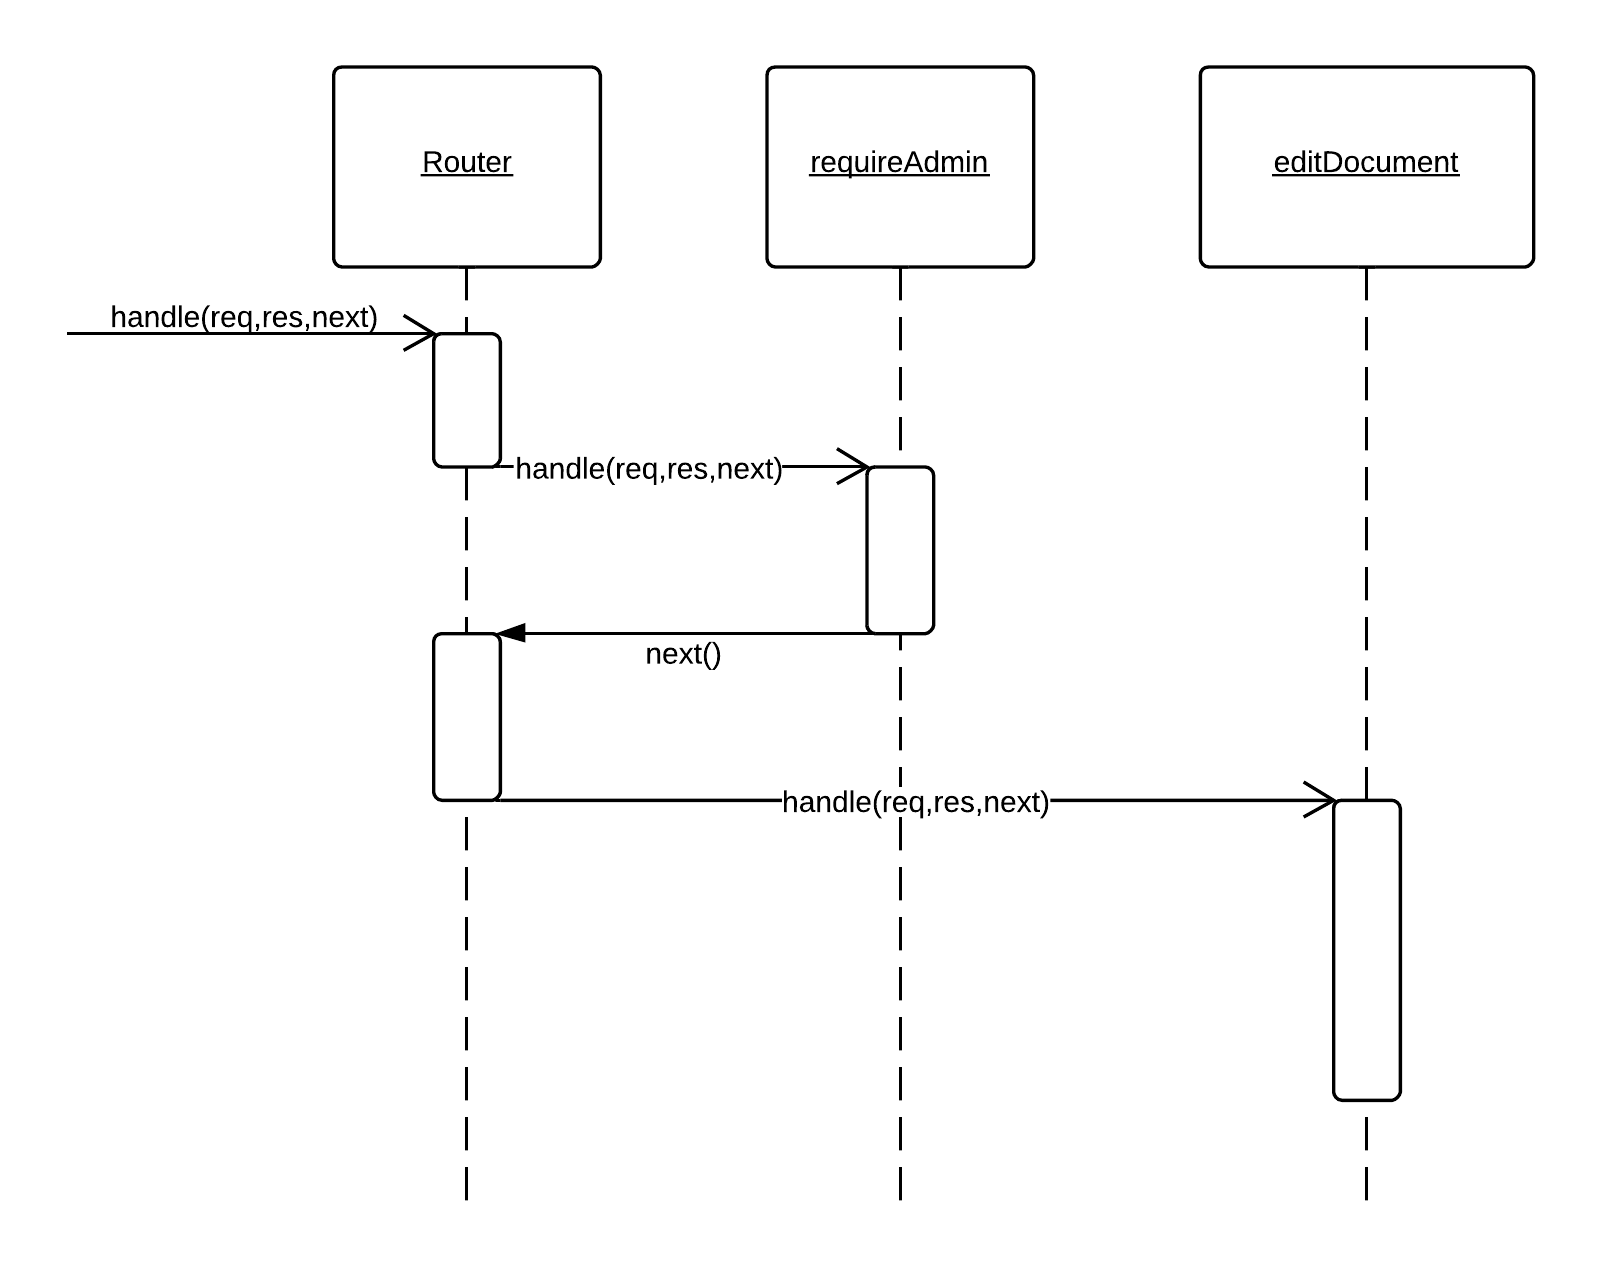
\includegraphics[scale=0.20]{scenari/Collection Name Document PUT.png} 
		\caption{Collection Name Document PUT}
	\end{center} 
\end{figure}

\subsubsection{Collection Name Document DELETE}
Il seguente scenario rappresenta la richiesta DELETE per una risorsa Collection name document, dopo che i permessi sono stati verificati il controllo è passato a \emph{deleteDocument} il quale gestirà la richiesta di eliminazione del document il cui id gli è stato passato come parametro.
\begin{figure}[H]
	\begin{center} 
		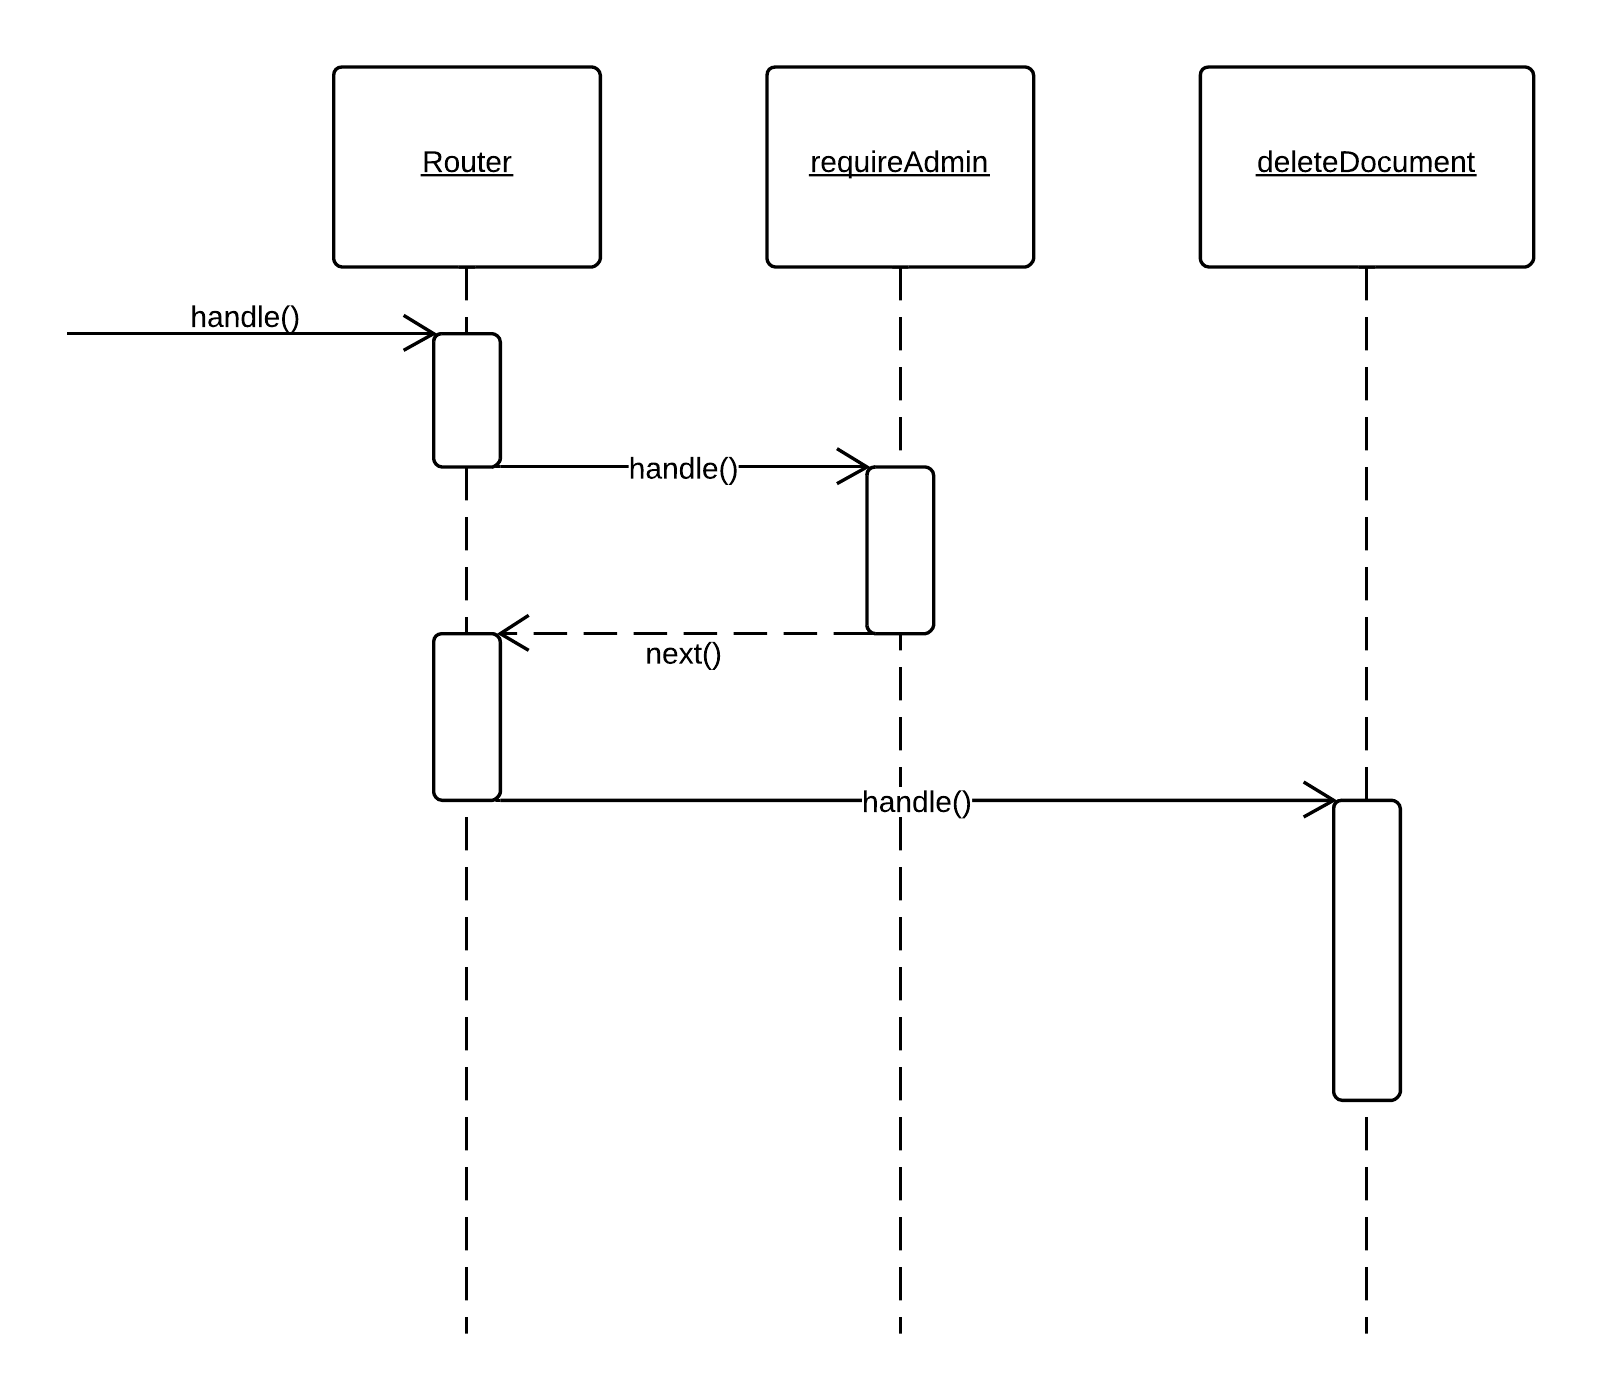
\includegraphics[scale=0.20]{scenari/Collection Name Document DELETE.png} 
		\caption{Collection Name Document DELETE}
	\end{center} 
\end{figure}

\subsubsection{Action Name Collection PUT} 
Il seguente diagramma di sequenza descrive lo scenario di una richiesta PUT per una risorsa Action name Collection.
Il controller \emph{collectionAction} si occupa di eseguire i controlli sugli attributi passatogli corrispondenti all'azione da eseguire e alla \glossario{Collection} sulla quale tale azione deve essere gestita.
\begin{figure}[H]
	\begin{center} 
		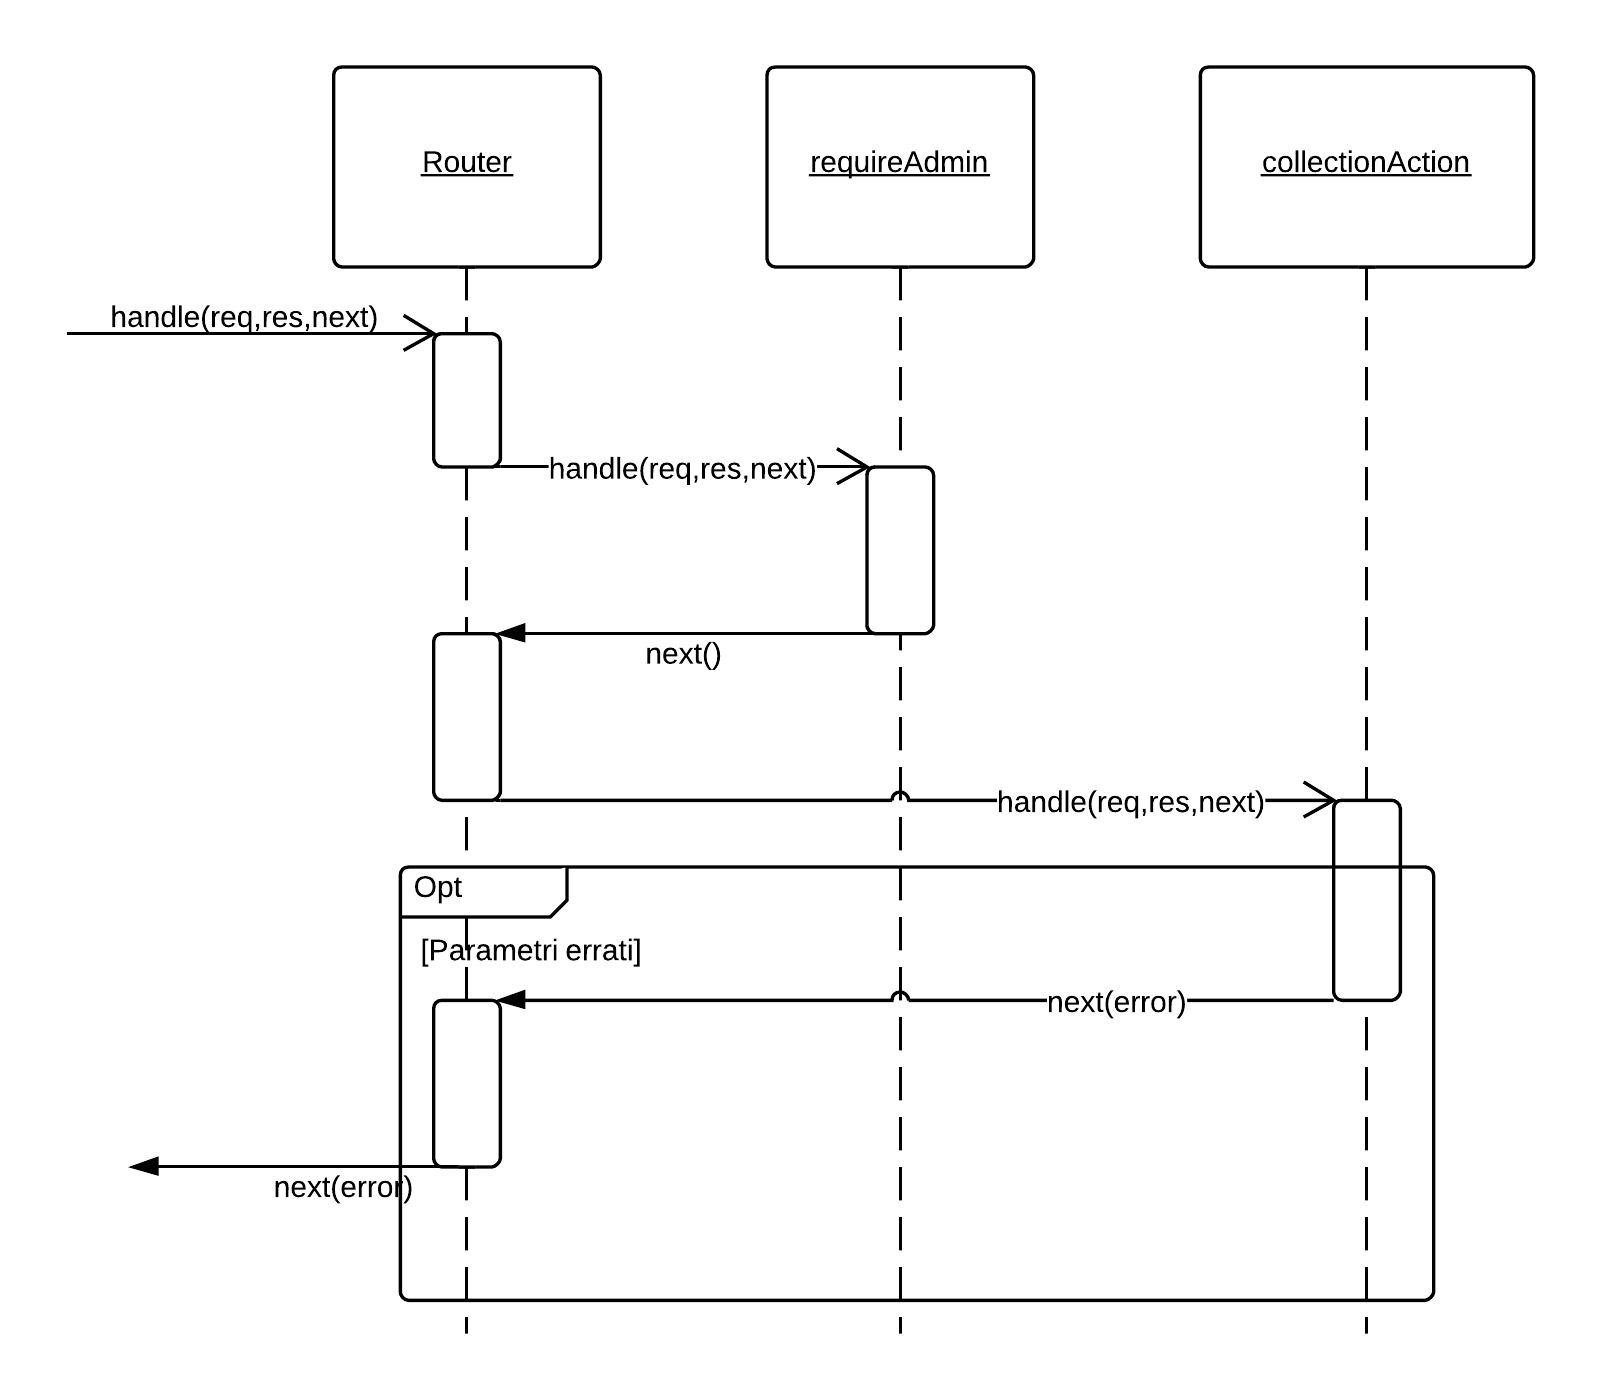
\includegraphics[scale=0.20]{scenari/Action Name Collection PUT.png} 
		\caption{Action Name Collection PUT}
	\end{center} 
\end{figure}

\subsubsection{Action Name Collection Document PUT}
Il diagramma a seguito mostrato descrive lo scenario di una richiesta PUT per la risorsa Action name Document.
Il controller \emph{documentAction} gestirà la richiesta di azione sul document corrispondente all'id passatogli come parametro.
\begin{figure}[H]
	\begin{center} 
		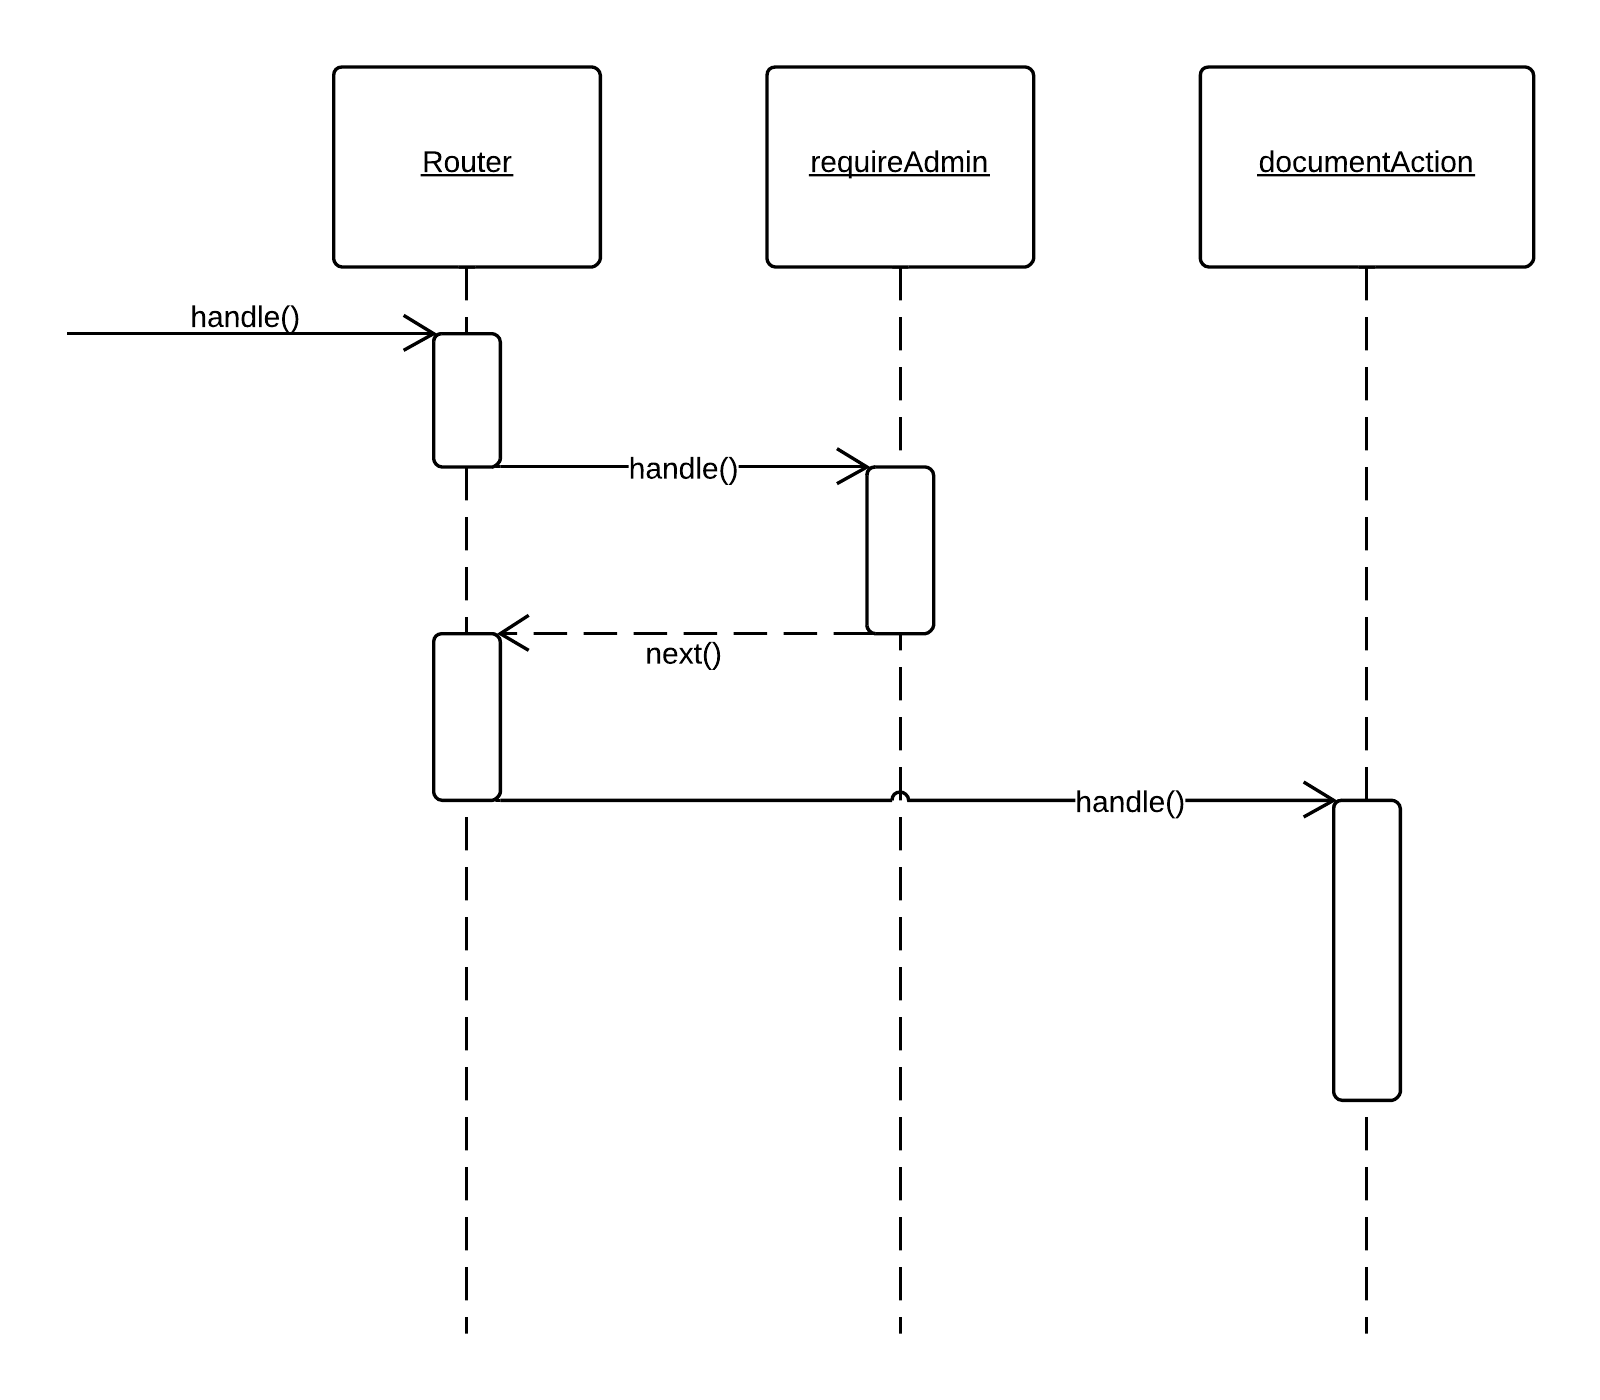
\includegraphics[scale=0.20]{scenari/Action Name Collection Document PUT.png} 
		\caption{Action Name Collection Document PUT}
	\end{center} 
\end{figure}

